%!TEX program = Traditional Builder with XeLaTeX
\documentclass[a4paper,12pt,oneside, fontset=mac]{ctexbook} % 使文档按单面打印模式排版
% \usepackage[UTF8]{ctex}
\usepackage{graphicx} % Required for inserting images
\usepackage{amsmath, amsthm, amssymb} % Math
\usepackage{wasysym} % Greek alphabets
\usepackage{unicode-math} % Greek alphabets, 替换MnSymbol. NOTE: 但只能在xelatex或者lualatex中使用
\usepackage{mathrsfs, amsfonts} % Math fonts
\usepackage{geometry} % Formatting
\usepackage{hyperref} % 引用链接
\usepackage{listings} % 代码输入
\usepackage{fancyhdr} % 引入fancyhdr宏包来控制页眉页脚
\usepackage{titlesec} % 定制章节标题样式
\usepackage{caption} % Optional, for caption customization
\usepackage{xcolor} % color
\usepackage{booktabs} % 使用booktabs表格形式
\usepackage{tabularx} % 在表格中制造换行
\usepackage{etoolbox} % 脚注通篇连续编号
\usepackage{xeCJK} % 控制字体
\usepackage[authoryear]{natbib} % 为了gbt7714加载natlib

% 设置页面边距
\geometry{
  a4paper,
  top=3.5cm, 
  bottom=2.5cm, 
  left=2.5cm, 
  right=2.5cm,
  headheight=2.5cm,
  footskip=2cm,
  bindingoffset=0cm
  }
\setlength{\oddsidemargin}{0pt} % 奇数页左边距偏移
\setlength{\evensidemargin}{0pt} % 偶数页左边距偏移

% 设置字体
\setCJKmainfont{SimSong} % 设置默认中文字体为宋体
\setmainfont{Times New Roman} % 设置默认英文字体为Times New Roman

% 设置chapter标题格式
\titleformat{\chapter}[block]
{\centering\zihao{3}\heiti} % 居中、三号、黑体
{\thechapter}
{1em}
{}
[\vspace{1ex}] % 段后空1行

% 设置chapter标题的前后间距
\titlespacing{\chapter}
{0pt} % 左边距
{1ex} % 段前空1行  
{1ex} % 段后空1行

% 重新定义section标题格式
\titleformat{\section}[hang]  % hang表示标题采用悬挂式样式
{\heiti\zihao{4}\raggedright}  % 黑体、四号、左对齐
{\thesection}{1em}{}  % 编号与标题间距1em

% 设置section标题的前后间距
\titlespacing{\section}
{0pt}  % 左边距
{1ex}  % 段前空1行
{1ex}  % 段后空1行

% 重新定义subsection标题格式
\titleformat{\subsection}[hang]  % hang表示标题采用悬挂式样式
{\heiti\zihao{-4}\raggedright}  % 黑体、小四号、左对齐
{\thesubsection}{1em}{}  % 编号与标题间距1em

% 设置subsection标题的前后间距
\titlespacing{\subsection}
{0pt}  % 左边距
{1ex}  % 段前空1行
{1ex}  % 段后空1行

% 脚注通篇连续编号
\counterwithout{footnote}{chapter} 

% 添加首行缩进,两个字符
\usepackage{indentfirst}
\setlength{\parindent}{2em}

% 设置行距
\renewcommand{\baselinestretch}{1.0}
\setlength{\parskip}{0pt}
\linespread{1.5}  % 固定行距20磅约等于1.5倍行距

% 避免出现所有作者名字
\usepackage[authoryear,etalmode=truncate,etaltext=it]{gbt7714}

% 设置页眉样式
\pagestyle{fancy}
\fancyhf{} % 清空默认页眉页脚
\fancyhead[C]{浙江财经大学硕士毕业论文}
\fancyfoot[C]{\thepage} % 居中显示页码

% document headings
\title{基于个人动态最优居住地选择视角的劳动力回流行为考察}
\author{Suicidal Bumblebee}
\date{Jan 2025}

\begin{document}

% 标题信息
\maketitle

\frontmatter
\renewcommand{\thepage}{\Roman{page}} % 将frontmatter页码改为大写罗马数字
% ---------------------------------------- 摘要 ----------------------------------------
\chapter{摘要}

\begin{center}
    \zihao{3}
    基于个人动态最优居住地选择视角的劳动力回流行为考察
\end{center}

随着经济的发展与社会工业化带来的社会关系剧变,劳动力迁移形成有规律的迁移模式是必然的。不同于我国研究中的传统城乡二元对立语境,本文基于理性预期构造了动态最优住址选择模型,基于CFPS数据对2010年至2022年间我国各省的人口流动进行实证检验,并得到的结论是(xxx、xxx、xxx)。本文的贡献在于(xxx、xxx、xxx)。

\textbf{关键词:} 动态迁移决策模型、劳动力迁移、收入引致、迁移摩擦


% ---------------------------------------- Abstract ----------------------------------------
\chapter{Abstract}

\begin{center}
    \zihao{4}
    \textbf{
    A Study of Return Migration Behavior Based on Dynamic Optimal Residential Location Decisions
    }
\end{center}

Here is the english version of abstract

\textbf{keywords}:a,b,c

% ---------------------------------------- 目录 ----------------------------------------
\thispagestyle{empty}
\tableofcontents

\mainmatter
% ---------------------------------------- 绪论 ----------------------------------------
\newpage
% \setcounter{page}{1} % 页码从此处开始记录
\chapter{引言}

% 点明人口流动的不均匀
纵观古今内外,“人往高处走,水往低处流”的规律总是屡试皆准。早在上世纪末,以\cite{krugmanIncreasingReturnsEconomic1991}和\cite{fujitaSpatialEconomyCities1999}为代表的新经济地理学就指出经济活动的集中会产生规模经济和网络效应,促成产业集聚。经济的聚集会导致区域不平衡发展,人们倾向于从“边缘”地区流向产业集聚、薪资较高和就业机会多的“中心”地区,形成“吸引效应”,这使得劳动力迁移有了移动的规律。欧美国家作为世界上人均GDP最高的区域,吸引大量来自其他相对落后国家的居民。根据世界银行(World Bank Group)和美国移民委员会(American Immigration Councile)公布的数据,
2023年美国的人均GDP为82769美元,外来人口达到了4780万,移民占美国人口的 14.3\%,比 1970 年的 4.7\% 增长了约三倍。相似地,在我国内部不同省份之间也发生着同样的人口迁移现象。改革开放以来,随着交通工具的进步和政策的放宽,劳动力自由流动在我国成为可能。解放的经济活力逐渐形成了“东富西穷、南富北穷”的局面。经济发展的不平衡不仅表现在地区收入差距上,也体现在人口分布的变化中。富裕地区吸引了大量来自相对贫困地区的劳动力。国家统计局2020年发布的《第七次人口普查》显示,流动人口达到3.76亿,占全国总人口比重分别为34.90\%和26.62\%,较2010年分别上涨88.52\%和69.72\%。
广东跨省流入高达2962.21万人,浙江也达到1618.65万人,上海跨省流入人口为1047.97万人。这三地的跨省流入人口数量位居前三。此外,北京流入841.8万人,位居第五。
同时,我国也存在多个人口输出大省\footnote{数据来源于2010年的《第六次人口普查》},例如
安徽省净向外输出约911万人,占本省户籍人口的13.29\%;
四川省净向外输出约956 万人,占本省户籍人口的10.63\%;
河南省净向外输出约约565万人,约占本省户籍人口的7\%。

% 介绍流动规律
在我国激烈的劳动力迁移浪潮中大致存在以下规律。
首先,劳动力净流入的区域符合常识中的迁移规律,劳动力从农村流向城市是迁移的主流趋势。大城市由于更高的工资水平、更丰富的就业资源、更高质量的基础服务设施,具有强大的“虹吸效应”,这一点与新经济地理学学者提出的观点相吻合。在可以预见的未来,这种劳动力向经济发达地区集中的趋势仍将持续。
其次,永久迁移与暂时性迁移之间存在显著差异。第七次人口普查显示,2020年时我国人户分离人口已达4.93亿,占总人口的34.16\%。(xxx)
并且,尽管总体上劳动力向发达地区流动,仍有部分劳动力“回流”到欠发达地区。这种反直觉的现象已被部分学者注意到(\cite{ShiZhiLeiJiaTingBingFuJiaTingJueCeYuNongCunQianYiLaoDongLiHuiLiu2012},\cite{RenYuanNongCunWaiChuLaoDongLiHuiLiuQianYiDeYingXiangYinSuHeHuiLiuXiaoYing2017}),表明某些群体在外迁后因各种原因选择返回原居住地,这揭示了迁移决策背后更为复杂的动机。
\cite{davanzoRepeatMigrationUnited1983}就指出过劳动力个体迁移行为的“反复无常”规律————尽管大多数个体从未迁徙,但迁徙的个体很可能会再次迁徙,通常会返回原籍地。这意味着迁徙决策应该被看作是一系列地点选择,个体知道有机会修改或逆转那些效果不佳的迁徙。

% 我国学术界对于劳动力研究存在不足
对于劳动力流动现象的研究,我国学术界长期围绕城乡二元分析框架与空间均衡模型展开。作为典型的发展中经济体,我国自计划经济时期形成的城乡二元结构构成了劳动力迁移的制度基础。改革开放后,工业化进程产生的劳动要素需求与农村剩余劳动力释放一拍即合,这一过程在学术研究领域直接映射为对传统二元经济理论的引用。其中,在\cite{lewisEconomicDevelopmentUnlimited1954}二元对立模型基础上,
\cite{todaroModelLaborMigration1969}通过引入失业率与预期收入,突破了无限劳动供给假设的刚性约束,其"即使存在失业风险,人口仍会因预期收入差距迁移"的核心命题,恰与中国城市化进程中农民工"候鸟式迁移"的特征契合,成为解释中国农民工流动现象的核心理论工具。而后,\cite{harrisMigrationUnemploymentDevelopment1970}进一步将城市正规部门与非正规部门纳入分析框架,通过工资刚性与就业概率的动态调整机制,构建起解释发展中国家城市失业与农村劳动力持续涌入并存现象的理论模型。这种强调制度分割与部门差异的分析视角,为中国学者解析户籍制度、土地制度等特殊约束条件下的劳动力流动提供了重要切入点。如\cite{XiongCaiYunNongMinGongChengShiDingJuZhuanYiJueCeYinSuDeTuiLaMoXingJiShiZhengFenXi2007}构建的农民工定居决策模型,通过引入城市拉力(就业机会、公共服务)与农村推力(土地保障弱化、收入差距)的交互作用,拓展了传统二元模型的解释维度。\cite{HuangZhongHuaNongCunTuDiZhiDuAnPaiShiFouZuAiNongMinGongShiMinHuaTuoDaLuoMoXingTuoZhanHeYiWuShiShiZhengFenXi2014}通过嵌入土地保险功能变量,\cite{ZhongShuiYingXiangChengRenKouLiuDongDeLiLunJieShiNongCunRenKouTuiChuShiJiaoTuoDaLuoMoXingDeZaiXiuZheng2015}纳入制度变迁因素。
部分文献虽然淡化了城乡之间的对立,但依然在均衡状态下分析工资和租金的确定,同时考虑移民流动对这些结果的影响。
\cite{ZongJiaFengDaChengShiZhiFuLiaoGengGaoDeGongZiMa2015}构建的三部门Rosen-Roback模型揭示,中国大城市存在显著工资溢价且技能异质性导致差异化集聚收益:高技能劳动力通过知识溢出获取短期增长红利,而低技能群体则需经历长期调整方能获益。
\cite{WangLiLiWoGuoRenKouQianYiChengBenChengShiGuiMoYuShengChanLu2020,WangLiLiTuDiGongGeiFangJieYuLaoDongLiKongJianPeiZhiXiaoLu2023,WangLiLiLaoDongLiLiuDongDuiChengShiGongZiYuFuLiDeYingXiangJiYuKongJianJunHengMoXingDeFenXi2024}通过将土地供给管制、迁移壁垒等制度变量内生化,定量识别出行政干预对劳动力空间配置的扭曲效应:建设用地指标的区域错配加剧东部大城市住房供给弹性不足,推高生活成本并阻碍生产率导向的人口集聚,导致2010年经济总产出损失达3\%-4\%。刘华仁(2024)则构建包含人力资本溢出效应的量化空间均衡模型,证明高技能劳动力的区域再配置可通过生产率与公共服务双重渠道提升社会福利,这为人才政策优化提供了理论依据。

% 逐渐引出动态方法
尽管现有研究取得显著进展,但传统劳动力迁移研究的局限性却愈发明显。首先,动态视角的缺位限制了理论的解释力。主流文献多依赖静态或比较静态分析,将迁移决策简化为单期最优选择,忽视了个体在生命周期内因人力资本积累、预期调整和制度环境变迁而产生的动态交互。例如,
\cite{HanQiHengNongCunLaoDongLiQianYiMoCaYingXiangNongMinGongShuLiangYuGongZiJieGouMa2018}虽尝试通过OLG模型捕捉迁移行为的代际动态,但其模型仍未能内生化制度约束与技能积累的交互效应。其次,微观基础的薄弱削弱了研究的政策适用性。许多研究基于宏观数据分析迁移的总体趋势,未能深入探讨个体异质性因素(如风险偏好、社会网络或数字技能)对迁移路径分化的影响,导致模型缺乏行为依据,难以支持精准的政策仿真。最后,理论范式的滞后使得现有模型难以适应劳动力流动的新特征。随着“城-城流动”规模扩大和远程就业的兴起,传统城乡二元对立的分析框架无法解释迁移的可逆性、多向性和地理重构效应。这些局限使得学界难以回答两个核心问题:在城乡融合发展和数字技术渗透的背景下,劳动力流动的长期均衡路径将如何演变?制度变迁如何通过重塑迁移的成本-收益结构影响个体的跨期决策?

针对上述问题,本研究提出从静态均衡向动态演化、从宏观相关性向微观行为基础、从单向城乡迁移向多维空间重构的理论转向。为此,本文构建了一个动态离散选择模型,将劳动力回流建模为一个马尔可夫决策过程(MDP)。该模型假设个体在有限生命周期内基于效用最大化原则选择居住地,效用函数综合考虑了地区吸引力(如工资和公共服务)、制度摩擦(如户籍限制)以及个体异质性(如乡土黏性和人力资本水平)。通过非参数混合估计方法,本研究量化以下机制:(1)户籍制度改革和土地确权如何通过提升预期稳定性增强迁移的持久性;(2)人力资本积累速率的差异如何导致迁移路径的分化,例如高技能个体更倾向于城市间的多次迁移;(3)远程就业的普及如何通过降低物理迁移成本重塑迁移的地理指向和频率。模型不仅为解析中国劳动力流动的复杂性提供了新的分析工具,还通过揭示迁移决策的微观驱动因素,为优化区域发展和以人为核心的城镇化政策提供了实证依据。

% 本文重要性、创新性等
本文的重要性在于,在当前工业化加速和经济转型的背景下,劳动力跨区域迁移问题愈发显得关键而复杂。人口流动不仅直接影响城市化进程、区域经济平衡和资源配置效率,还对社会福利和经济结构的长期调整产生深远影响。尤其在中国这一快速发展的经济体中,劳动力回流现象既是城市化进程的缩影,也是城乡协调发展的关键变量。深入理解和准确预测劳动力迁移趋势,不仅有助于把握经济发展的内在动力,还为政策制定提供了科学依据,以实现区域协调发展和社会整体进步。

本研究从动态决策的视角切入,系统分析劳动力回流的规律及其驱动机制,特别强调收入差异作为核心经济因素的作用。与此同时,模型综合考虑了就业机会、生活成本、制度摩擦和文化因素的交互效应。例如,户籍制度作为中国特有的制度约束,可能通过限制公共服务获取提高迁移成本,从而影响个体是否选择永久定居城市。同样,地区间的文化差异(如方言)可能通过乡土黏性影响迁移决策的稳定性。通过构建理论模型并结合实证分析,本文旨在回答以下问题:地区间的收入差异如何激发劳动力迁移?收入差异如何与其他因素(如公共服务供给和户籍限制)共同作用于迁移决策?通过何种政策干预可以引导劳动力合理流动,从而优化资源配置、促进城乡协调发展并提升社会福利?

正如\cite{desmetUrbanAccountingWelfare2013}在城市规模与福利分析中所指出的,理解决定人口分布的各种力量对于回答一系列关键问题至关重要:这些力量在决定城市规模分布中的相对重要性如何?如果各地区在公共服务、技术水平或制度摩擦方面趋于一致,人口将如何重新配置?这种重新配置对社会福利的总体影响是什么?这一论述启发本研究将收入差异置于更广泛的动态框架中,探讨其如何通过影响迁移决策重塑人口分布和区域经济格局。如果地区间的制度和经济差异缩小,劳动力流动和城市规模分布可能发生显著变化,进而影响整体社会福利。本研究通过量化这些机制,为劳动力迁移的理论和实证分析提供了一个综合框架。

% 结构安排
为实现上述研究目标,本文结构安排如下:第二章对国内外相关文献进行系统综述,梳理劳动力迁移的理论演进和实证成果,分析现有研究的不足,并明确本文的创新点。第三章构建动态离散选择模型,详细阐述模型的基本假设、机制设计以及与现实经济现象的关联,推导劳动力迁移存在性的理论命题。第四章推导实证分析所需的似然函数,说明模型简化的必要假设(如支撑点离散化处理未知分布),并介绍数据来源(中国家庭追踪调查和地区年鉴)、变量构造和Python实现的计算方法。第五章展示实证分析的主要结论,通过对不同样本子集的检验和命题验证,评估模型在解释中国劳动力回流中的适用性和稳健性。第六章总结研究的主要发现,讨论模型的局限性(如理性人假设的适用性、函数形式的潜在任意性),并提出未来研究方向,例如引入收入分配结构或跨省迁移的网络分析。
此外,更为详细的数学证明、程序代码和数据处理流程均附在文末的附录中。



% ---------------------------------------- 文献综述 ----------------------------------------
\chapter{文献综述}

劳动力流动作为经济社会发展的重要表征,其研究要点在于提供合适的方法和寻找符合现实逻辑的影响因素。本文通过系统梳理国内外近几十年来的经典文献与前沿成果,试图厘清学术脉络的演进逻辑,为后续实证研究提供标准。
在研究方法层面,现有文献呈现出从静态分析向动态追踪的范式转变。就影响因素而言,学者们已逐步突破传统经济变量的单一解释,将制度约束、社会网络、文化认同等非经济维度纳入分析体系。

\section{历史线索}
\label{sec:_历史线索}

%定义回流问题到我们的研究问题

劳动力回流通常指出于某些原因曾经迁出的劳动力又返回原籍地。
这种迁移现象可撤回的(retractable),也可以被视作是短暂的(temporary)。对于迁移的决策者来说,这种迁移肯定不是一次性的,这也正是传统静态方法所难以刻画的。

劳动力回流问题的研究有以下几个特点。

首先,
劳动力回流问题是一个出现时间较短的问题。
从人类社会发展进程来看,工业化历史仅延续数百年,大规模人口迁移现象的存续时间更为有限,
而规模化的劳动力返迁现象就更加以观察。

其次,
传统人口流动模式呈现显著单向性,即遵循从经济欠发达地区向经济发达地区的转移规律。这一现象已通过社会认知固化成为了一种社会常识,刻印在我们的直觉中。
即便在目标地存在显著负外部性(如工业化时期伦敦、巴黎等城市的环境污染问题),人口仍持续向城市集聚以获取生存空间和发展机会。
劳动力回流现象最难以理解的部分在于————
当目标地发生经济衰退致使预期收益低于原籍地时,返迁决策符合理性选择理论预期;
然而当目标地仍能提供显著的收入溢价时,劳动力仍选择返迁,这一现象与传统理论预测产生背离,从而构成了值得深入探究的理论悖论。

再次,劳动力回流现象的研究对于后发工业化国家具有更重要的政策意义。  
在自由迁移的经济体系中,劳动力的区位选择本质上是区域经济一般均衡的衍生结果。劳动力的空间分布受到地区间发展差异的影响,并通过市场机制实现最优配置,从而促进社会整体福利的最大化。
但是正如\cite{CaiFangHuJiZhiDuYuLaoDongLiShiChangBaoHu2001}等学者所强调的,对于处于全球发展金字塔中部及中后部分的后发国家而言,政府为加速资本积累和工业化进程,通常会实施非均衡发展战略。这种战略通过制度化的城乡二元结构,人为压低农产品相对价格并抬高工业品价格,形成工农产品价格剪刀差。
这种政策实质上是将农业剩余通过隐蔽税收机制向工业部门进行强制性转移,从而导致资源从传统农业部门向现代工业部门的系统性倾斜。
\footnote{
  设经济分为农业部门A和工业部门M,其产出分别为农业产出\( Y_A = F_A(L_A, K_A, T) \)和工业产出\( Y_M = F_M(L_M, K_M) \) ,其中\( L_A, L_M \) 为两部门劳动力,\( K_A, K_M \) 为两部门资本,\( T \) 为土地(农业部门特有)。

  政府通过政策压低农产品价格 \( P_A \),抬高工业品价格 \( P_M \),使得交换比价 \( \frac{P_A}{P_M} \) 低于市场均衡水平。设市场均衡价格为 \( \frac{P_A^*}{P_M^*} \),政策扭曲后\(\frac{P_A}{P_M} < \frac{P_A^*}{P_M^*}\) 。农业剩余\(S_A = Y_A - C_A\)是农业产出超过农民自身消费的部分,其中 \( C_A \) 为农业部门的基本消费需求。  

  由于价格剪刀差,农业剩余以低价被转移至工业部门,工业部门获取的额外收益(相当于对农业的隐性征税)为\(T_{implicit} = (P_A^* - P_A) \cdot Y_A\)。这部分剩余被用于工业投资的资本积累,\(I_M = T_{implicit} = (P_A^* - P_A) \cdot Y_A\)。
}
同时,后发工业化国家通常需要将大量劳动力集聚于城市区域以支撑现代化生产体系,并通过将农业部门剩余劳动力向现代工业部门转移,为资本原始积累提供廉价人力资源供给。
\footnote{
  在城乡对立经济中,由于\(\frac{\partial Y_M}{\partial L_M}>0\)总成立。
  政府通过政策控制迁移速率 \( \mu(t) \),使得农业劳动力被迫向工业部门转移,即
  \(\dot{L}_M = \mu(t) \cdot L_A - \rho L_M\)与\(\dot{L}_A = -\mu(t) \cdot L_A + \rho L_M\),
  其中\( \mu(t) \) 是政府控制的迁移率(如强制招工、限制返乡),\( \rho \) 是劳动力自发回流率(通常被政策压制,\( \rho \approx 0 \))。政策目标是维持 \( L_M \) 持续增长,防止 \( L_A \) 回升。

  工业部门的工资由劳动力供需决定\(w_M = \eta \cdot \frac{Y_M}{L_M}  - \lambda \cdot (L_M - L_M^*)\)。其中\( \eta \) 是劳动生产率系数,\( L_M^* \) 是市场均衡劳动力规模,\( \lambda \) 衡量劳动力过剩对工资的压制效应(\( \lambda > 0 \))。

  由于政府人为维持 \( L_M > L_M^* \),导致\(w_M \text{ 被压低,且 } \frac{\partial w_M}{\partial L_M} < 0\)。
  通过人为制造劳动力过剩(\( L_M \gg L_M^* \)),压低工资以维持出口竞争力,复制了东亚的人口红利优势增长路径。
}
如果劳动力选择逆向回流至原籍地,将不利于后发国家的资本深化与工业化进程。
因此,后发工业国家的学术研究往往带有明显的政策导向性(例如\cite{QuanZhuoWeiWoGuoNongCunShengYuLaoDongLiZhuanYiDeYanJiu1996}等学者的研究)——如同牧场主将羊群迁往他们想要赶去的地方一样,其核心聚焦于如何通过政策与制度安排将农村剩余劳动力集中配置至城市部门,人为制造当地劳动力市场供过于求的状态,从而抑制工资上涨,为劳动密集型工业品生产创造持续的廉价人力资本优势。这一机制正是包括我国在内的东亚及东南亚经济体在上世纪后半叶实现快速工业化,并逐步缩小与欧美国家经济差距的关键基础。农村村剩余劳动力的转移是经济发展的必然趋势。

但是与日韩港台等东亚模式的不同之处在于,在实现快速工业化之前,我国已确立社会主义基本制度。这使得我国的工业化具有社会主义国家工业化路径的特殊性,即在计划经济向市场经济转型过程中,国家通过公有制主导、产业政策引导及劳动力市场管制等制度安排,形成了独具特色的国家主导型工业化模式。

在上世纪50到80年代期间,由于工业基础薄弱、生产能力严重不足,全国上下都面临典型的"短缺经济"困境,为了维持国家的稳定和政党的统治,在资源分配上我国实施了严苛的管制制度————在微观层面实行粮油票证制度,通过配额制保障基本生活物资分配;在宏观上,则是建立起了以户籍制度为核心的空间资源配置体系。
产生生这一现象的原因在于,由于发展工业化的资源极其缺乏,其本质是工业化初期面临的“资本原始积累约束”,这使得国家不得不
通过行政手段将有限资本集中配置于几个少数城市,这一时期北京、上海、天津等城市,出于在地理、政治、经济上独特的优势条件,获取大量的资源,从而形成医疗、教育等公共服务的高度集聚。
但如果不对这些稀缺资源实施准入限制,就会出现严重的资源挤兑、资源稀释和搭便车问题,这正是户籍制度产生的深层经济逻辑。该制度的部分功能延续至今,仍在特定领域发挥着制度惯性作用。

在改革开放之后,我国吸取资本主义制度中关于市场经济的成功经验,借鉴东亚发展型国家的成功经验,通过市场机制培育工业化所需的物质基础。
这一转型过程需要大规模农村劳动力向工业部门转移,特别是在2001年加入世界贸易组织后,我国明确采取出口导向型发展战略,主动承接全球价值链中的劳动密集型环节,充分发挥人口红利的比较优势。\cite{LinYiFuZhongGuoDeJingJiFaZhanZhanLueYuDiQuShouRuChaiJu2003}为所阐述的新发展经济学理论,为这一发展路径提供了系统的理论支撑。

正是在这个快速工业化、快速现代化的历史进程中,
大量的人口或被鼓励、或自主地涌入了城市,
形成了我们如今熟知的人口迁移文化:
沿海发达地区凭借其经济优势持续吸纳内陆欠发达地区的剩余劳动力,而若干核心城市群则逐步演变为国民经济活动的主要空间载体。
然而,在这场深刻重塑我国社会经济地理格局的人口大迁徙中,却呈现出显著的逆向迁移现象。现有研究表明,我国劳动力市场中存在明显的回流特征,这一现象与后发国家工业化进程中的劳动力配置目标存在理论上的背离。
具体到本文研究的语境,
劳动力回流是指劳动力从相对贫穷地区迁出又迁回,对于我国来说
这种问题大量表现为:
农村居民进程打工形成农民工,
但是在若干时间之后又返回原籍,
形成农民工返潮现象。

在快速工业化的世界中,快速发展经济的社会潮流与维持社会稳定的政治制度在效率上起了难以调和的矛盾。
随着社会资源逐渐丰富了起来,
上层建设却逐渐与社会基础脱离。
仅就发展社会经济而言,许多社会制度存在着大量的社会主义残余,首当其冲的就是户籍制度。

不少学者的研究结果指出,户籍制度障碍可能是影响劳动力定居的首要因素。我国对户籍制度进行了大量的改革,但是仍存在难以完全取缔的系统性障碍。例如,\cite{RenYuanChengShiLiuDongRenKouDeSheHuiRongHeWenXianShuPing2006}指出以户籍制度为依托的流动人口管理制度 以 及一系列与户口相关的社会福利制度对流动人口的限制与排斥 对流动人口的社会融合有着根本性 的影响,而
\cite{LuYiLongHuKouHuanQiZuoYongMaHuJiZhiDuYuSheHuiFenCengHeLiuDong2008}认为即使经历了大量深刻的改革,户籍制度仍然对劳动力自由流动造成客观上的阻碍。
这种制度刚性在一定程度上阻碍了劳动力要素的优化配置,构成了制约经济高质量发展的重要制度因素。

还有部分观点认为,劳动力回流问题可能是由于我国在实现快速现代化中另一项政策的导致的,即土地财政。
土地财政的源头来源于1994年的分税制改革。彼时,中央与地方财权重新分配,地方政府税收收入占比下降,但承担的事权未减少。同时,改革开放后,大量农村人口涌入城市,催生了对土地开发和房地产的巨大需求。
面临捉襟见肘的财政盈余,土地成为地方政府自主掌控的重要资源。
从此,地方政府依靠土地出让金、土地税费等土地相关收入作为财政收入的重要来源。这种独特央地关系下的财政模式就是土地财政。
对于经济发展而言,
地方政府通过征收农村土地,转变为建设用地后出让给开发商,土地出让金成为地方政府预算外收入的重要来源,土地抵押融资支持基础设施建设。
由于政府是土地的完全垄断者,按照最基本的经济学原理,垄断者必定会降低供给、提高价格从而实现利润最大化。
垄断性质的土地出让金提供了大量资金支持城市基础设施建设,成为地方政府投资驱动型增长的重要工具,
但是也造成了地方政府有动力维持较高地价,进而推高房价,造成部分城市房价与居民收入严重脱节,
增加了居民家庭的住房负担,形成"高杠杆"现象。\cite{ChenYingFangNongMinGongZhiDuAnPaiYuShenFenRenTong2005,niehuihuaZhongguogaofangjiadexinzhengzhijingjixuejieshiYiZhengqihemou2013,YuJianXingDiFangFaZhanXingZhengFuDeXingWeiLuoJiJiZhiDuJiChu2012}等学者的观点就支撑该观点。

特别是在大城市中,由于存在巨量人口,但是住房供给过低,使得居住成本成为市民的难以企及的负担。
因此部分学者认为,住房不平等的加剧影响社会阶层流动性,是导致劳动力回流的最根本原因。
\footnote{
  设政府是建设用地的唯一供给者,土地供给量 \( L_s \)由政府控制。土地需求 \( L_d \) 由房地产开发商决定,取决于房价预期和开发利润\(L_d = D(P_h, r)\)其中\( P_h \) 为房价,\( r \) 为融资成本。
  政府作为垄断者,通过选择 \( L_s \) 来最大化土地出让收入\(\max\limits_{L_s}  P_L(L_s) \cdot L_s \),其中 \( P_L(L_s) \) 是土地价格,由供需决定\( P_L(L_s) = \frac{\partial P_h}{\partial L_s} \cdot \frac{P_h}{\text{弹性}} \)。
  房价 \( P_h \) 由土地成本、建筑成本和开发商利润构成$P_h = P_L \cdot \theta + C_b + \Pi_d$,其中\( \theta \) 是容积率(单位土地上的住房面积),\( C_b \) 是建筑成本,\( \Pi_d \) 是开发商利润。

  由于政府限制土地供给(\( L_s \ll L_d \)),土地价格 \( P_L \) 被推高$P_L = \frac{a}{L_s^b} \quad (a>0, b>0)$(即土地供给越少,价格越高)。

  令居民购房支出占收入比重为$\beta = \frac{P_h \cdot H}{Y}$,其中\( H \) 为住房面积,\( Y \) 为居民收入。
  当 \( \beta > \text{警戒值}\) 时,居民必须增加杠杆(负债)
  $\text{家庭杠杆率 } \lambda = \frac{D_h}{Y} \quad \text{(} D_h \text{为住房负债)}$
  在大城市,人口 \( N \) 远高于土地供给弹性,而住房供给 \( S_h = \theta L_s \) 受限,产生了住房供需失衡:
  \[
  \frac{S_h}{N} \downarrow \implies P_h \uparrow \implies \beta \uparrow \implies \lambda \uparrow
  \]
  过重的负担会导致劳动力无法承担居住成本从而回流。
}

在户籍与地价两大历史线索之外,还存在着其他不同的可能研究方向,例如:
原籍地经济发展,就业机会增加,工资差距缩小,生活成本差异变化;
家庭纽带和亲情牵引,文化认同和归属感,社会融入困难,子女教育需求等;
户籍制度改革,公共服务可及性变化,返乡创业政策激励,流入地歧视政策或制度障碍。
这一部分内容将留到本章\ref{sec:_影响劳动力迁移的因素}小节中进行进一步讨论。
以上是对于劳动力回流问题的历史脉络探索,
接下来本文对研究劳动力流动的两种主要方法进行梳理和对比,并根据分析选择最优的方法。

\section{空间均衡方法}

本文采取的方法实则将迁移决策视作选择序列,在介绍这种方法之前,同样重要的是了解其互为补充的方法,即空间均衡方法。根据\cite{jiaEconomicsInternalMigration2023}的研究,通常有两种方式来研究劳动力迁移问题。第一种方法,如前所述,是空间均衡方法。
该方法认为在迁移行为之后必然存在新的空间一般均衡。在这种理念下,研究者检视人口流动是如何影响各种变量的出清,例如本地工资、不同地区的房价等因素。
\footnote{
一个基本的空间均衡模型可以由以下设定给出。
假设经济中有 $N$ 个地区,每个地区的劳动力市场和住房市场都满足一般均衡条件。设$ L_i $ 表示第 $ i $ 个地区的劳动力数量(人口);$ W_i(L_i) $随着劳动力供给递减的工资函数;$ H_i(L_i) $ 表示房价函数,假设其为劳动力供给的增函数。

劳动力迁移是基于个体效用最大化的决策行为。假设个体效用 $ U_i $ 是工资和房价的函数:$U_i = f(W_i, H_i)$,其中 $ f(\cdot) $ 是一个效用函数,通常假设工资对效用有正向影响,而房价对效用有负向影响。
劳动力迁移会导致不同地区的劳动力分布发生变化,从而影响工资和房价。在新的均衡状态下,所有地区的个体效用应趋于一致(否则会有进一步的迁移)。即
$U_i = U_j \quad \forall i, j$,
这一条件可以写成
$f(W_i(L_i), H_i(L_i)) = f(W_j(L_j), H_j(L_j)) \quad \forall i, j$。

在新的均衡状态下,劳动力市场的供给和需求必须出清。假设第 $ i $ 个地区的劳动力需求由生产函数决定:$L_i^d = g(W_i)$,
其中 $ g(\cdot) $ 是一个递减函数(工资越高,企业雇佣的劳动力越少)。
劳动力市场出清条件为:$L_i^s = L_i^d \quad \forall i$,即:$L_i = g(W_i(L_i)) \quad \forall i$。
类似地,住房市场的出清条件可以表示为$H_i(L_i) = h(L_i)$,其中 $ h(\cdot) $ 是住房供给函数。

将上述条件整合起来,整个模型可以写成联立方程组
$\begin{cases}
f(W_i(L_i), H_i(L_i)) = f(W_j(L_j), H_j(L_j)) \quad \forall i, j \\
L_i = g(W_i(L_i)) \quad \forall i \\
H_i(L_i) = h(L_i) \quad \forall i
\end{cases}$,
这些方程共同决定了劳动力迁移后的空间均衡状态,包括各地区的劳动力分布 $ \{L_i\} $、工资水平 $ \{W_i\} $ 和房价水平 $ \{H_i\} $。
}

经济学中的空间均衡概念可以追溯到20世纪中叶,\cite{samuelsonSpatialPriceEquilibrium1952}提出了一个简称“空间价格均衡”(Spatial Price Equilibrium)框架,其中考虑运输成本,调整不同地点的价格以平衡供需。这项工作奠定了空间经济学的基础,最初侧重于商品市场,但后来也为后来应用于劳动力和移民提供了概念基础。
\cite{tieboutPureTheoryLocal1956}提出了著名的用脚投票(vote by feet)理论,Tibeout假设在一个没有迁移成本且信息完全的经济体中,消费者可以自由地在不同地点之间移动,选择最能满足其偏好模式的社区;也就是说,他们“用脚投票”。\cite{harrisMigrationUnemploymentDevelopment1970}提出了一个两部门的内部贸易模型,研究农村到城市的迁移,其中城市的最低工资高于农村收入。当城市部门的预期工资(即经失业调整后的实际工资)等于农村部门的平均工资时,达到均衡。

受城市经济学发展的影响,劳动力市场和区位选择的转变始于20世纪60年代和70年代。
由William Alonso、Richard Muth和Edwin Mills在20世纪60年代开创的单中心城市模型,考察了城市内部的空间结构,重点关注通勤和住房选择。
虽然该模型主要研究城市内部,但它通过强调空间因素如何影响经济决策,为城市间移民研究奠定了基础。
一项关键性的进展来自\cite{rosenHedonicPricesImplicit1974},该文给出的享乐定价模型基于观察到的价格和属性对差异化产品的特征(包括区位)进行估值。这种方法对于移民研究至关重要,因为它使经济学家能够通过观察特定地点的便利设施(例如气候、犯罪率和服务获取)对工资和租金的影响来量化这些设施的价值。
在Rosen模型的基础上,\cite{robackWagesRentsQuality1982}正式确立了有关移民的空间均衡模型。Roback将享乐模型扩展到一般均衡环境,假设个人会迁移到能够获得最高效用的地点,同时考虑金钱因素(工资、租金)和非金钱因素(便利设施)。在均衡状态下,没有人能够通过迁移来提高效用,因为工资和租金会进行调整,以平衡不同地点的效用。该模型成为基础模型,尤其适用于理解便利设施如何影响移民模式和城市增长。

继Roback的研究之后,空间均衡方法在20世纪80年代和90年代得到了显著扩展,以适应更为复杂研究需求。学者们纳入了例如住房市场动态、非贸易商品以及多种类型的主体等因素。在这之中,住房供应弹性的纳入变得至关重要,正如\cite{glaeserWealthCitiesAgglomeration2009}中所强调的那样,他们指出,城市的成功可以体现为人口增长或收入增长,具体取决于住房供应状况。
扩展模型还包括考虑迁移成本和移民异质性的模型,正如在Roback框架基础上构建的后续研究中所见。这些发展使我们能够更细致地理解移民流动,尤其是在应对区域经济差异和政策变化方面。
\cite{glaeserWealthCitiesAgglomeration2009}以及\cite{morettiLocalLaborMarkets2011}概述了一些重要例子。
例如,\cite{morettiLocalLaborMarkets2011}提出了一个一般均衡模型,假设工人的流动性不一定是无限的,因为对某些地点的特殊偏好,住房供应也不一定是固定的。
另一种衍生模型涉及多部门或多类型工人的模型,允许偏好和技能的异质性。该模型已被用于研究城市内部的不平等和隔离等问题,考察不同群体如何基于其经济资源竞争理想的位置。
例如\cite{diamondDeterminantsWelfareImplications2016}估计了一个结构性空间均衡模型,研究技能分类增加的原因及其福利影响。
\cite{coen-piraniEffectHouseholdAppliances2010}开发了一个动态一般均衡模型,强调个体异质性在迁移决策中的作用。

在过去二十年中,空间均衡方法已被整合到定量空间模型中,通常被称为定量空间经济学(quantitative spatial economics)。
例如\cite{ahlfeldtEconomicsDensityEvidence2015}和\cite{reddingQuantitativeSpatialEconomics2017},这些研究扩展了 Rosen-Roback 框架,引入了市场准入项,提供了内生价格作为基本面和地理因素函数的对数线性方程(定量空间模型),使其能够更好地捕捉现代经济的复杂性。这些模型对于政策分析尤其有用,可以评估基础设施投资或移民政策对空间经济结果的影响。

空间均衡模型的动态版本也已出现,研究城市如何随时间演变以及移民如何应对冲击。一个值得注意的例子是\cite{glaeserHousingDynamicsUrban2014},它继承了Alonso、Rosen和Roback的传统,构建了一个动态的、线性的、理性的一般均衡模型,并与住房市场的典型事实(例如建设持续性和价格均值回归)相一致。
该方法已应用于国际移民研究,如\cite{albertImmigrationSpatialEquilibrium2022},该文记录了移民如何受原籍国支出的影响而聚集在生活成本高昂的城市,并使用定量空间均衡模型评估其对生产力的影响。

如上所述,动态空间均衡模型是另一种衍生模型,它捕捉收入冲击或政策变化等时变因素。表格 \ref{tab:_history of spatial equilibrium on migratory problem} 清晰的展示了空间均衡方法的发展历史。

\begin{table}[!ht]
\centering
\caption{使用空间均衡方法研究人口流动的历史}
\label{tab:_history of spatial equilibrium on migratory problem}
\begin{tabularx}{\textwidth}{@{}lX@{}}
\toprule
\textbf{时期} & \textbf{关键发展}\\
\midrule
\textbf{1950年代} & Samuelson引入了空间价格均衡,通过运输成本平衡不同地点的供需。奠定了空间均衡经济学的基础,但最初侧重于商品市场。\\
\textbf{1960-1970年代} & Alonso、Muth和Mills等开发了关注通勤和住房选择的城市内模型,影响了城际移民研究。为区位选择提供了空间框架,为移民应用奠定了基础。\\
\textbf{1970年代} & Rosen建立了享乐定价模型,通过工资和租金等观察到的价格来评估区位属性(例如便利设施),能够量化区位选择中的非金钱因素,为移民研究奠定了基础。 \\
\textbf{1980年代} & Roback正式建立了一个一般均衡模型,其中工资、租金和便利设施使不同地点的效用均衡,从而解释了移民模式。成为研究移民的基石,将经济激励与区位决策联系起来。\\
\textbf{1980-1990年代} & Glaeser与Gottlieb等将住房供应弹性、非贸易商品和异质性主体纳入模型。通过解决住房动态和不同的移民偏好增强了现实性。\\
\textbf{2010年代} & Redding, Rossi-Hansberg, Ahlfeldt 等人整合市场准入和贸易成本,扩展 Rosen-Roback 模型,使用对数线性方程对工资和人口进行建模。改进了基础设施和贸易对移民影响的政策分析。\\
\textbf{近期} & 拓展:国际移民、信息约束、多部门和异构代理模型 \\
\bottomrule
\end{tabularx}
\end{table}

近年来,我国学术界通过空间均衡模型对人口流动及劳动力资源配置进行了深入研究,探讨了其在区域发展、城市化及社会福利优化中的作用。例如,
\cite{LiangRuoBingDiFangGongGongPinGongGeiZhongDeTieboutMoXingJiYuZhongGuoChengShiFangJieDeJingYanYanJiu2008}基于Tiebout模型,通过动态面板回归模型检验了35个中国大中型城市的住房价格与地方公共品供给之间的关系。
\cite{LiuHuaRenLiZiBenKongJianPeiZhiDeSheHuiFuLiXiaoYingYanJiuJiYuLiangHuaKongJianYiBanJunHengMoXingDeFenXi2024}构建了一个包含异质性劳动力生产率溢出和公共服务溢出的空间一般均衡模型,分析人力资本空间配置优化的社会福利效应及可行政策。其研究表明,优化人力资本空间配置可显著提高社会福利,特别是通过再分配政策促进高技能人才向低工资城市的均衡分布,能够实现帕累托改进。
\cite{WangLiLiWoGuoRenKouQianYiChengBenChengShiGuiMoYuShengChanLu2020}结合空间均衡模型与地级市数据,研究人口迁移对劳动力资源配置及城市规模的影响。
\cite{WangLiLiTuDiGongGeiFangJieYuLaoDongLiKongJianPeiZhiXiaoLu2023}进一步分析土地供给政策对劳动力空间配置效率的影响。研究表明,政府对建设用地指标的管控决定了住房供给弹性,东部大城市的严格规制导致房价高涨,阻碍人口向高生产率地区转移,加剧了劳动力资源的空间错配。放松东部大城市的土地利用规制,有助于改善劳动力配置效率并减少经济产出损失。
\cite{ZhaoFangZhongGuoChengShiHuaFaZhanJiYuKongJianJunHengMoXingDeYanJiu2017}基于\cite{diamondDeterminantsWelfareImplications2016}的模型,引入户籍和土地供给规则,探讨中国劳动力迁移的微观机制。研究发现,工资水平仍是影响迁移的主要因素,但对于流动人口,城市舒适度也起到重要作用。此外,高、低学历劳动力之间存在互补性,但劳动力市场回报更偏向高学历劳动力,房价则主要受迁移人口增减影响。

虽然空间均衡方法影响深远,但也并非没有受到批评。一些人认为,诸如完全流动性和同质主体等假设可能过于简化了现实世界的复杂性。此外,该模型对均衡条件的依赖可能无法完全捕捉短期迁移动态或社会网络和文化因素的作用。
同时,空间均衡方法在宏观情况下可能很有效,但在微观数据上却有困难,需要非均衡方法作为补充。
接下来本文将介绍空间均衡方法的补充————微观视角方法。


\section{个体微观视角与动态选择方法}

与空间均衡方法所审视的宏观均衡不同,存在着一种考虑个体视角的研究方法。类比来说,这相当于交通道路模拟中的元胞自动机微观方法,而上述方法相当于流体力学宏观方法。

个体视角的劳动力流动研究可以视作从\cite{sjaastadCostsReturnsHuman1962}开始。Sjaastad提出了一个模型,假设个人根据迁移的成本和回报做出地点决策。回报包括货币回报以及基于位置偏好的非货币回报。
这种观点实际上将移民视为一项投资,强调了移民的动态方面——移民的预期成本和收益会随着时间的推移而变化。
从生命周期的角度来看,个人(或家庭)决定是否以及何时移民。前期做出的决策(例如储蓄、教育、婚姻、生育)决定了当前时期的选择,对未来事件的预期也会影响当前的决策。从这个角度来看,移民和生育选择通过决策过程的“原始要素”联系在一起:当前机会(部分由过去的决策决定)、期望(预期的未来事件和结果)和偏好(分配给不同结果的值)。因此,微观视角的研究方法提供了一个统一的框架将几种重要的现实行为联系起来。

\cite{mincerFamilyMigrationDecisions1978} 开发了一个模型来允许家庭联合移民决策,认识到家庭的最佳地点选择可能与个人配偶的最佳地点选择不同。

在接下来的 40 年里,这些模型在许多重要维度上得到了扩展,包括效用函数、时间范围和位置选择集等因素。2011 年著名的\cite{kennanEffectExpectedIncome2011}提出的个人移民选择模型结合了许多这些进步。
该文中的结构动态模型允许个人进行丰富的决策过程。它允许个人技能和位置偏好的异质性,以及迁移成本的异质性。它还允许许多备选位置选择,每个位置的收益流通常不确定,允许工资和偏好的位置匹配成分,允许连续的位置决策而不是单一选择。该模型将个人移民决策作为最佳搜索过程来解决,旨在描述工人对不同地点工资差异的局部均衡反应,假设个人最大化预期终生收入,扣除迁移成本。
该模型的重要贡献之一就在于将动态离散选择模型结合到移民问题考察中,将移民问题视作了最优居住地选择问题。

动态离散选择(Dynamic discrete choice, DDC)理论遵循单个决策主体动态的研究模式。
当DDC模型用于迁移问题研究时。
它是为了分析个体或家庭如何在多个创业居住地之间做出最优化选择的模型,考虑各种经济、社会、地理和政策因素,以解释人口迁移、城市发展和住房市场的动态。其背后的基本思想是,当迁移迁移的净预期收益超过时,个人会选择迁移迁移假设迁移是对外部冲击或永久性工资增长机会的响应,从而提高个体的有效使用水平。
一个标准的DDC具有如下基本特征:
离散时间序列中的动态性;
单个决策者面临多个、有限、离散、完整且可分离的选择;
无论选择与否,选择都不会被淘汰;
马尔可夫决策过程。这意味着仅有T-1期的状态变量影响T期,而不是更前期;
不确定性,或者说随机决策环境;
显示偏好和微观数据。

毫无疑问,DDC是研究动态迁移决策过程最合适的工具。
迁移目的地是广阔的、有限的、离散的和可分离的。
个人或家庭都可以视为单个决策者,决策者在离散时间序列的每个时期做出的动态迁移选择,
由于在整个时间序列中始终存在选择,因此这种理论可以用于描述可撤回的迁移行为。

离散选择模型在经济学和社会科学中至关重要,用于分析有限选项之间的决策。
该理论的源头来源自\cite{thurstoneLawComparativeJudgment1927}提出了一种通过成对比较来测量心理价值的模型,即从心理激励的角度引入了比较判定定律 (Law of Comparative Judgment)。
定律指出具有真实激励水平的选择项$i$被感知含有一个正态误差,即$V_i+\epsilon_i$,其中\(\epsilon_i\)为正态误差。假设该误差独立同分布,这与二元概率模型相符,为决策分析提供了理论基础。
基于Thurstone的洞见,经济学家在20世纪中期将离散选择模型形式化。
\cite{marschakBinarychoiceConstraintsRandom1960}将这种感知到的刺激$V_i+\epsilon_i$解释为效用 并对包含随机因素的效用最大化的选择概 率进行了理论上的推导。Marschak 将其称为随机效用最大化 (Random Utility Maximization, RUM) 模型。这一效用模型是如今所有离散选择模型的理论基础。
而后,\cite{mcfaddenConditionalLogitAnalysis1973}引入了条件逻辑模型,将二元逻辑模型扩展到多种替代方案。该模型对运输经济学至关重要,它允许选择概率依赖于替代方案的属性,从而确立了离散选择作为一种标准的计量经济学工具的地位。同时,多项概率模型和嵌套逻辑模型等模型解决了诸如不相关替代方案独立性(IIA)属性等局限性。

学者逐渐意识到静态模型不足以应对具有跨期依赖性的决策,这促使动态离散选择模型的发展。 离散选择模型的动态性深深植根于动态规划的发展,这是\cite{bellmanDynamicProgramming1957}中提出的一个概念。Bellman 的工作为解决序列决策问题提供了数学框架,是马尔可夫决策过程 (Markov Decision Process, MDP) 的基础。 
\cite{blackwellDiscreteDynamicProgramming1962}进一步推进了这一研究,在离散环境中为 MDP 建立了理论基础,这是DDC 模型的核心。
到 20 世纪 80 年代初,MDP 已在微观和宏观经济理论、金融和运筹学中得到广泛应用,包括\cite{arrowOptimalInventoryPolicy1951}的最优库存政策、\cite{lucasInvestmentUncertainty1971}的不确定性下的投资等。这些研究虽然并非 DDC 的独有,但为将动态规划应用于经济学中的离散选择问题奠定了基础。

经济学中的 DDC 模型领域开始于 20 世纪 80 年代中期,\cite{pakesPatentsOptionsEstimates1986}将专利续展决策建模为动态离散选择问题,使用随机控制模型估计持有专利的价值,这突出了模型在处理不确定性和离散选择方面的效用。
\cite{rustOptimalReplacementGMC1987}经常被引用为开创性著作。它提供了经济学中最早的实证应用之一,为公交公司维护主管 Harold Zurcher 是否更换巴士发动机的决策过程建模。这项研究建立了一个无限期模型,包含了状态转换和随机冲击,引入了嵌套不动点 (Nested Fixed Points, NFXP) 算法进行最大似然估计,成为该领域的经典示例。
这之后,后续应用有\cite{wolpinEstimableDynamicStochastic1984}在生育率和儿童死亡率方面的应用、\cite{millerCultureDevelopmentEveryday1984}在工作匹配方面的应用以及\cite{pakesPatentsOptionsEstimates1986} 在专利续展方面的应用,证明了该模型的多功能性,正如\cite{aguirregabiriaDynamicDiscreteChoice2010}所言。
\cite{ecksteinDynamicLabourForce1989}则提出并估计了一个已婚女性劳动力参与率和生育率的动态模型,明确考虑了工作经验对工资的影响。研究表明,尽管工作经验会增加未来工作的负效用,但这种影响被经验对工资的正效应所抵消,从而维持了女性的就业模式。此外,子女数量和丈夫收入的增加显著降低女性的劳动力参与率,而教育水平的提高则对其参与率产生显著正向影响。
\cite{keaneStructuralEstimationBehavioral2011}系统介绍了离散选择动态规划(DCDP)模型的结构估计方法,并探讨了其在劳动经济学中的重要贡献。文章以典型的女性劳动力参与模型为例,详细阐述了DCDP模型的求解与估计方法,并回顾了其在劳动力供给、求职行为和人力资本积累等三大前沿领域的应用。


由于需要反复求解动态规划问题,估计动态离散选择模型的计算量巨大。
为了缓解这一问题,\cite{hotzConditionalChoiceProbabilities1993}引入了条件选择概率方法。这种方法避免了为每个参数猜测求解完整动态规划问题的需要,大大提高了计算可行性,并成为一种可行的非解估计方法(non-solution method)。
模拟方法(例如模拟矩法)以及近期方法,例如 \cite{suConstrainedOptimizationApproaches2012}提出的带均衡约束的数学规划 (MPEC),进一步减轻了计算负担。
这些改进,包括处理未观测到的异质性和序列相关性,增强了模型的真实性和可行性。
表格\ref{tab:不同作者对于动态离散选择模型的贡献}总结了DDC模型中方法论的关键发展。

\begin{table}[!ht]
\centering
\caption{不同作者对于动态离散选择模型的贡献}
\label{tab:不同作者对于动态离散选择模型的贡献}
\begin{tabularx}{\textwidth}{@{}cXX@{}} 
\toprule
\textbf{年份} & \textbf{作者} & \textbf{贡献}\\
\midrule
1987年 &John Rust &开发了嵌套不动点 (NFXP) 算法,这是一种用于估计的全解方法。开创性的公交车发动机更换模型,经典示例。\\
1993年 &V. Joseph Hotz、Robert A. Miller &开发了条件选择概率,这是一种领先的无解估计方法。\\
1994年 &V. J. Hotz、R. A. Miller、S. Sanders、J. Smith &提出了一种计算更简单的条件选择概率版本,并在公交车发动机更换上进行了测试。\\
2012年 &Che-Lin Su、Kenneth Judd &使用 Artelys Knitro 实现了约束优化 (MPEC) 方法进行估计。 \\
2016 年 &Fedor Iskhakov、Jinhyuk Lee、John Rust、Bertel Schjerning、Kyoungwon Seo &结果表明,MPEC 相对于 NFXP 的速度优势并不显著,NFXP 在马尔可夫决策模型中仍然保持领先地位。\\
\bottomrule
\end{tabularx}
\end{table}


过去十年,研究重点在于融入现实的行为假设并拓展应用。例如,\cite{utaraDynamicDiscreteChoice2024}探讨了动态不一致性问题,并将该模型应用于2011年东日本大地震期间的疏散选择。另一篇\cite{heckmanDynamicDiscreteChoice2007}将动态选择模型与处理效应估计相结合,增强了政策分析能力。计算能力的进步使得具有高维状态和多智能体的模型成为可能,并应用于卫生经济学、环境经济学和市场营销领域。


国内对于DDC的研究较少,
多数集中在对于机制的探讨。
例如\cite{QinSongDongTaiChiSanXuanZeMoXingJiQiGuJiFangFaFaZhanZongShu2010}和\cite{MaYaQiDongTaiChiSanXuanZeMoXingDeMoNiFenXi2016}对于DDC的原理和方法给出了介绍和讨论。


如\cite{jiaEconomicsInternalMigration2023}所说,使用DDC模型探劳动力迁移问题在本质上是一种非均衡方法。这与空间均衡方法截然不同。两者代表了两种不同的分析范式,其差异本质上是宏观均衡分析与微观行为分析的分野。
它们在理论基础、研究视角、方法工具和应用场景等方面存在显著差异。
例如,空间均衡方法植根于新古典经济学的一般均衡理论,强调区域间要素的联动调整与市场出清机制。当区域间存在工资、房价或公共服务差异时,劳动力和企业会通过迁移或调整投资行为,最终使各区域的效用和利润趋于均等化,形成无套利均衡状态。
而基于DDC的最优居住地选择模型则以微观经济学的效用最大化理论为基础,聚焦个体在异质性偏好下的决策过程。个体通过比较不同区位的预期效用(如收入、生活成本、就业机会、环境质量等),选择能实现终身效用最大化的居住地。
空间均衡方法采用宏观视角,关注城市或区域层面的整体均衡状态。这种视角的优势在于揭示系统性规律,但可能忽略微观个体的异质性行为。最优居住地选择模型则采用微观视角,聚焦个体或家庭层面的决策过程。这种视角的优势在于捕捉个体异质性,但难以直接反映宏观均衡效应。
空间均衡方法依赖区域层面的汇总数据,常用结构方程或联立方程系统进行估计。例如,通过校准区域间工资方程和住房供给函数,反推隐含的迁移成本或偏好参数。最优居住地选择模型需要微观个体数据(如人口普查、家庭追踪调查数据),常用离散选择模型(如条件Logit、嵌套Logit)或机器学习方法。例如,利用中国家庭追踪调查(CFPS)数据,估计农民工市民化决策中收入、教育、社会资本的边际效应。两种研究方法的不同之处如表格\ref{tab:空间均衡方法与个体选择方法的对比}总结所示。

\begin{table}[!ht]
\centering
% \renewcommand{\arraystretch}{0.8} % 压缩行间距到 80%
\caption{空间均衡方法与个体选择方法的对比}
\label{tab:空间均衡方法与个体选择方法的对比}
\begin{tabularx}{\textwidth}{@{}lXX@{}} 
\toprule
\textbf{比较维度} & \multicolumn{1}{c}{\textbf{空间均衡方法}} & \multicolumn{1}{c}{\textbf{最优居住地选择模型}} \\ \midrule
理论基础 & 基于新古典经济学一般均衡理论,强调区域间要素的联动调整、均衡状态和市场出清 & 基于效用最大化理论,强调个体决策和行为微观基础,是局部均衡视角下的产物 \\
代表模型 & Tiebout模型、Rosen-Roback模型 & 动态离散选择模型、Logit计量模型、推拉模型 \\
研究视角 & 关注城市/区域层面的整体均衡状态 & 聚焦个体/家庭的最优决策过程 \\
核心假设 & 完全流动性、完全信息 & 效用最大化、异质性偏好 \\
时间维度 & 多为静态或比较静态分析,关注长期均衡 & 可以进行动态分析,关注短期和长期迁移决策 \\
均衡作用 & 侧重于个体和企业在不同地点之间无差异的空间均衡条件 & 均衡是个体选择的结果,但重点在于决策过程本身 \\
异质性处理 & 弱异质性,通常假设同质性劳动力或有限异质性 & 强异质性,明确建模个体异质性和偏好多样性 \\
内生性处理 & 通过均衡条件内生确定工资、房价等 & 通过计量方法处理迁移决策中的内生性问题 \\
计量方法 & 结构方程估计、联立方程系统 & 离散选择模型、条件Logit、嵌套Logit、混合Logit \\
政策应用 & 适合评估宏观政策对要素价格和人口分布的影响 & 可模拟个体行为响应(如迁移补贴对不同收入群体的激励差异) \\
数据需求 & 依赖区域层面汇总数据(平均工资、房价、失业率) & 需要微观个体数据(人口普查、家庭追踪调查) \\
预测能力 & 预测区域间总体流动趋势 & 预测个体迁移行为和选择概率 \\
典型应用 & 区域经济收敛性研究,税收与公共服务匹配分析 & 农民工市民化决策预测,高技能人才跨国流动研究 \\
局限性 & 忽略个体决策异质性 & 微观模型难以反映系统均衡效应 \\ 
\bottomrule
\end{tabularx}
\end{table}


显然,劳动力回流问题需要设计一个可以刻画暂时性迁移的框架,在这方面微观方法更胜一筹。

\section{对回流迁移的研究}

通常我们强调国内与国外文献的融合,但在劳动力回迁问题上,国内国外在具体议题上存在较大不同。具体而言,在我国独特国情下,劳动力回流问题指的都是农民工返潮现象,而国外研究大致都是研究在一个自由流动的背景下劳动力如何自由选择的。在这个前提下,我们有必要先对国内外的学术工作分开进行总结,接着再从国外文献的研究方法中汲取有用的共性以服务于国内研究课题。


国外关于劳动力回流(return migration)的研究重点关注自由流动背景下个体和家庭如何在不同地点间进行迁移决策。与我国不同,国外研究通常聚焦于国际移民的往返迁移、临时性迁移及其经济和社会驱动因素。

早期研究如\cite{gmelchReturnMigration1980}综合了南欧、东欧和加勒比地区的案例,指出20世纪初欧洲移民中有四分之一返回原籍国。
\cite{wymanRoundtripAmericaImmigrants1993}则通过历史记载分析了1880-1930年间从美国返回欧洲的移民,归因于怀旧情绪和本土主义怨恨等因素。这些研究奠定了对回流迁移现象的基本理解。

\cite{sjaastadCostsReturnsHuman1962}首次将移民定义为一种人力资本投资,强调个人在预期回报超过成本时选择迁移。这一静态框架为后续研究提供了基础,但其局限性在于无法处理多目的地选择问题。\cite{tunaliRationalityMigration2000}尝试扩展至动态框架,但仍局限于二元选择。
\cite{dierxLifecycleModelRepeat1988}则结合面板数据,分析家庭人力资本分布对迁移决策的影响,弥补了单期模型的不足。
\cite{dahlMobilityReturnEducation2002} 通过罗伊模型探讨了自我选择迁移机制,解释了美国劳动者高流动性与地区教育回报差异之间的关系。\cite{gemiciFamilyMigrationLabor2007}进一步构建包含家庭内部协商的动态模型,发现家庭纽带会抑制人口流动性并减缓工资增长。
在以上早期模型的基础上,\cite{kennanEffectExpectedIncome2011}他们利用全国青年纵向调查(NLSY)中针对高中教育白人男性的面板数据,开发了一个动态离散选择模型,该模型允许在多个备选方案中进行最优的地点决策序列。该模型通过考虑收入前景来捕捉回归移民,发现地域工资差异和对更佳地点匹配的追求会影响决策,包括在当前收入不利的情况下回归。这标志着一项重大进展。
在这之后,
\cite{dustmannEconomicsTemporaryMigrations2016}强调了临时迁移的重要性,提出一个通用理论框架,分析技能积累、技能回报率差异及消费偏好如何驱动跨国往返迁移。研究表明,即使缺乏外生冲击,这些内生机制仍能引致回流行为。\cite{venatorDualEarnerMigrationDecisions2022}整合家庭动态和空间因素,改进估计技术,推动了该领域方法论的进步。


国内关于劳动力回流的研究主要集中在农民工返潮现象,分析其影响因素及经济社会效应。然而,现有研究多停留在静态选择框架下,采用简单的Logit或Probit回归模型进行实证分析。
\cite{WangZhiQiangZhongGuoNongCunLaoDongLiQianYiYingXiangYinSuYanJiuJiYuProbitMoXingDeShiZhengFenXi2011}利用中国健康与营养调查(CHNS)数据,通过Probit模型分析了农村劳动力迁移决策的影响因素。研究表明,婚姻状况、健康水平和娱乐偏好等变量显著影响迁移决策,而当前收入的作用不明显。此外,已婚女性倾向于与配偶共同迁移,这种行为加剧了农村“空巢老人”问题。研究还发现,提高教育水平是促进农村劳动力迁移的最有效手段,尤其是高等教育和职业教育。
\cite{ShiZhiLeiJiaTingBingFuJiaTingJueCeYuNongCunQianYiLaoDongLiHuiLiu2012}基于湖北和河南两省的农户调查数据,利用Multinomial Logistic模型探讨了家庭禀赋对农村迁移劳动力回流的影响。研究发现,家庭人力资本和社会资本在不同阶段对迁移决策产生差异化影响:人力资本丰富的家庭更倾向于让劳动力留在或回流农村,但当人力资本达到一定水平后,劳动力又更愿意外出就业;社会资本则在初期促进外出务工,但在高水平时推动劳动力回流。此外,家庭经济资本兼具收入效应和替代效应,总体上更倾向于促使劳动力回流。
\cite{RenYuanNongCunWaiChuLaoDongLiHuiLiuQianYiDeYingXiangYinSuHeHuiLiuXiaoYing2017}以外出劳动力是否发生回流为因变量,构建Logistic模型分析回流迁移的影响因素。研究表明,城市就业排斥、经济收入不足以及社会保障缺失是推动劳动力回流的重要原因,同时家庭生活需求、农业活动和农地状况也对回流决策产生显著影响。研究进一步指出,回流迁移是“被动回流”与“主动回流”的结合,体现了个体决策与家庭决策的综合过程。回流不仅带来人力资本补偿,还促进了流出地非农经济发展和创业增长,成为城镇化过程中不可或缺的逆向迁移流。


如同先前指出,
静态框架下理论模型无法涵盖迁移的暂时性和可撤回行,难以捕捉迁移的动态特征和复杂性。
相比之下,国外文献中广泛应用的动态离散选择模型能够更好地刻画迁移的暂时性和可撤回性。
因此本文鉴国际经验,结合动态离散选择模型方法与回流问题探讨我国劳动力回流的驱动机制及其经济社会影响。

\section{影响劳动力迁移的因素}
\label{sec:_影响劳动力迁移的因素}

为了将 DDC 模型扩展为更有用的实证工具,必须系统整合迁移决策理论的相关研究成果。

在迁移决策理论的发展脉络中,\cite{leeTheoryMigration1966}提出的"推-拉"理论(Push-Pull Theory)具有奠基性意义。该理论构建了二元分析框架:推力因素(如经济萧条、社会动荡、环境恶化等负向激励)促使个体离开原居地,而拉力因素(如就业机会、公共服务、环境品质等正向吸引)则驱动个体流向特定目的地。这一理论范式为迁移决策的多元影响因素分析提供了系统性思路。
想要实现尽可能客观的研究,就必须要在DDC模型中和推拉模型一样考虑足够多的影响因素。
在\ref{sec:_历史线索}中,本文对于户籍制度和土地财政导致的房价高企问题进行了简答的描述,但是想要刻画一个劳动力流动模型,我们需要从更客观的角度出发,思考种种可能因素。
DDC模型的优势在于其能够通过随机效用函数的结构化设定,将多维决策因素纳入迁移行为的分析框架。
这种多维度的建模思路,正是DDC模型相较于传统迁移分析方法的理论优势所在。

\textbf{房价}作为影响劳动力流动的重要因素,在中国居高不下且持续增长的背景下,成为学术界关注的核心议题。
\cite{GaoBoQuYuFangJieChaiYiLaoDongLiLiuDongYuChanYeShengJi2012}基于2000-2009年中国35个大中城市的面板数据发现,相对房价的提高会促使劳动力流出,并对低附加值产业产生挤出效应,进而引发产业升级。房价上涨显著增加了农村劳动力的生活成本,对其进入城市形成阻碍(高波等,2014)。类似地,\cite{WangLiLiTuDiGongGeiFangJieYuLaoDongLiKongJianPeiZhiXiaoLu2023}结合空间均衡模型与地级市数据指出,东部大城市的严格土地规制导致住房供给缺乏弹性,高房价阻碍了劳动力向高生产率地区的转移,加剧了空间错配。
\cite{ZhouYingGangGaoFangJieJiChuLiaoShuiJiYuZhongGuoLiuDongRenKouDeWeiGuanShiJiao2019}从个人层面分析发现,高房价增强了劳动力家庭的流动意愿,特别是对未购房的高技能劳动力具有显著挤出效应。尽管公共服务在一定程度上缓解了高房价的负面影响,但大城市中的挤出效应尤为突出。此外,已购房产的劳动力更倾向于流向房产所在地,而住房财富效应则推动劳动力向省会及以上城市迁移。
\cite{zhouHousingPricesMigration2022}通过引入住房成本自选择模型,结合2017年中国流动人口动态调查(CMDS)数据,发现高房价显著抑制了低技能流动人口的就业积极性。研究表明,房价每上涨1\%,流动人口的平均受教育年限增加0.297年,表明高房价对低技能劳动力形成挤出效应,同时促进了高技能劳动力的正向选择。这种现象在租房或自购住房的年轻流动人口中尤为明显,尤其是那些有意定居移民城市的群体。
\cite{ZhangLiFangJieRuHeYingXiangLaoDongLiLiuDong2017}从理论和实证角度论证了房价对劳动力流动的双重作用:一方面,高房价作为城市特征信号降低了未来收入的不确定性,吸引人才流入;另一方面,快速上涨的房价压缩了可支配收入,加重了外来劳动力的生活成本,从而抑制其流入。这种拉力与阻力的综合作用使得房价对劳动力流动呈现先吸引后抑制的倒U型影响。\cite{LiHuiFangJieFangJieShouRuBiYuLiuDongRenKouChangQiJuLiuYiYuanLaiZiLiuDongRenKouDeWeiGuanZhengJu2019}指出房价对流动人口长期居留意愿影响不显著,房价收入比对流动人口长期居留意愿存在显著负影响。
\cite{ballHousingSupplyPrice2010}和\cite{helpmanSizeRegions1998}的研究提供了国际视角。前者指出,尽管高房价地区抑制劳动力流入,但预期套利机会仍可能吸引部分劳动力;后者强调经济集聚推高房价的同时,房价也反过来抑制劳动力进一步集聚,揭示了房价与劳动力流动之间的双向互动关系。


\textbf{户籍制度}也是我国劳动力流动的重要制度性障碍,近年来学术界围绕其对城市化进程、城乡收入差距及劳动生产率的影响展开了广泛探讨。
\cite{ngaiChinasMobilityBarriers2019}指出,我国户籍制度通过绑定公共福利(如教育、医疗等)和社会转移支付限制了人口流动,同时土地政策导致农业就业过剩,阻碍了工业化进程。研究表明,建立有效的土地使用权保障和竞争性租赁市场可缓解这一低效现象,而地方社会转移支付的限制对工业化的负面影响较小。
\cite{LiQiangYingXiangZhongGuoChengXiangLiuDongRenKouDeTuiLiYuLaLiYinSuFenXi2003}进一步分析发现,户籍制度使中国的人口流动不再遵循传统的推拉规律。长期的制度约束改变了农民工的心理预期和生活目标,削弱了推力和拉力的作用,形成了独特的迁移模式。
\cite{LuYiLongHuKouHuanQiZuoYongMaHuJiZhiDuYuSheHuiFenCengHeLiuDong2008}利用OLS方法分析了户籍制度对社会流动的影响,强调其在加剧社会分层中的作用。\cite{tombeTradeMigrationProductivity2019}通过一般均衡模型量化了户籍政策带来的高迁移成本,发现2000年至2005年间,国内贸易和人口迁移成本的下降贡献了总劳动生产率增长的36\%。尽管成本有所降低,但户籍壁垒仍然显著,尤其是大城市对劳动力进入的限制,导致城市化滞后于工业化,城市规模不足,制约经济发展(\cite{WangLiLiWoGuoRenKouQianYiChengBenChengShiGuiMoYuShengChanLu2020})。因此,进一步放松户籍限制被认为是提升城市化水平和资源配置效率的关键。
\cite{ZhouWenTuDiLiuZhuanHuJiZhiDuGaiGeYuZhongGuoChengShiHuaLiLunYuMoNi2017}在刘易斯二元经济模型基础上引入土地流转和户籍限制,分析了两者对城市化、要素价格及居民福利的影响。研究表明,土地控制和户籍限制共同抑制了劳动力流动,而改革这些制度有助于提高城市化水平并缩小城乡收入差距。\cite{AnHuSenChengShiGaoFangJieHeHuJiZhiDuCuJinHuoYiZhiChengXiangShouRuChaiJuKuoDaZhongGuoLaoDongLiLiuDongHeShouRuChaiJuKuoDaBeiLunDeYiGeJieShi2011}则结合新经济地理学模型,探讨了城市高房价与户籍制度对城乡收入差距的“门槛效应”。研究发现,当城乡市场开放度较低时,高房价扩大收入差距,而户籍制度起到抑制作用;但当市场开放度超过某一临界值时,户籍制度反而加剧了收入差距,此时废除户籍制度才能促进城乡协调发展。
现有研究表明,户籍制度和土地政策通过多种机制影响劳动力流动及其经济后果。一方面,它们通过增加迁移成本、限制公共服务获取等方式抑制人口流动,导致城市化滞后和资源错配;另一方面,其对城乡收入差距的影响具有非线性特征,需结合市场开放度等因素具体分析。未来研究应进一步探索如何通过制度创新和政策优化降低迁移壁垒,释放劳动力市场的潜在生产力,推动城乡协调发展。


在社会学和经济学研究中,\textbf{舒适度}(amenity)是影响人口迁移的重要因素。这些变量包括空气质量、公共服务水平、城市天气等,共同塑造了劳动力的空间流动模式。
\cite{YangXiChengShiGuiMoYuChengZhenHuaNongMinGongShiMinHuaDeJingJiXiaoYingJiYuChengShiShengChanLuYuYiJuDuChaiYiDeDingLiangFenXi2017}定量分析了城市生产率和宜居性对劳动力流动的影响,发现城镇化显著提升了实际GDP和城乡劳动力的实际工资,但其效应因城市规模而异。农民工市民化在中小城市(人口300万以下)可能导致经济效率下降,而在中等城市(人口100万-300万)则对农村劳动力福利提升最为显著。\cite{WangLiNuoJiYuYaLiMenJianJiaShuoDeJiaTingQianJuYiXiangXingChengJiZhiYanJiuYiHangZhouShiQuWeiLi2007}基于Rosen-Roback的空间均衡理论指出,收入、生活成本(如房租)和城市宜居性特征共同决定了劳动力的空间流动模式。

\cite{XiaYiRanChengShiJianDeMengMuSanQianGongGongFuWuYingXiangLaoDongLiLiuXiangDeJingYanYanJiu2015}研究表明,公共服务(如教育和医疗)显著影响劳动力流向,长期流动人口更倾向于选择公共服务水平较高的城市。然而,公共服务的作用系数仍小于工资水平对迁移决策的影响,因此政策制定者需科学评估公共服务均等化的实际效果。\cite{GuoDongMeiChengXiangRongHeDeShouRuHeFuLiXiaoYingYanJiuJiYuYaoSuPeiZhiDeShiJiao2023}通过一般均衡模型进一步分析了户籍制度改革、公共服务均等化和土地市场一体化的联动效应,强调单一市场的改革可能造成部分群体福利受损,而综合改革能有效缩小城乡差距并提升整体福利。\cite{LiuJinFengChengShiGongGongFuWuDuiLiuDongRenKouYongJiuQianYiYiYuanDeYingXiang2019}利用2017年中国流动人口动态监测数据发现,城市公共服务显著增强流动人口的永久迁移意愿,尤其是对城镇流动人口和第一代农民工的影响更为突出。

城市能提供的福利也是宜居度的重要组成部分。\cite{benjaminImportingPoorWelfare2004}通过比较边境县与内陆县的AFDC参与率,发现高福利地区的吸引力显著高于低福利地区。\cite{mckinnishWelfareinducedMigrationState2007}进一步扩展了这一研究,发现尽管大多数估计值统计上不显著,但短距离迁移在福利移民流动中具有重要性。\cite{degiorgiWelfareMigrationEurope2009}探讨了欧盟扩大前各国的福利移民问题,发现福利慷慨程度对移民决策有显著但较小的影响,这种影响足以扭曲移民流动分布。

\cite{SunWeiZengKongQiWuRanYuLaoDongLiDeKongJianLiuDongJiYuLiuDongRenKouJiuYeXuanZhiXingWeiDeYanJiu2019}利用条件Logit模型分析了空气污染对流动人口就业选址行为的影响,发现PM2.5浓度每上升1μg/m³,流动人口到该城市就业的概率下降0.39个百分点。年龄较大、受教育水平较高以及男性、已婚/已生育的流动人口对空气污染更为敏感。\cite{ZhangYanKongQiWuRanDuiBenDiLaoDongLiLiuChuDeYingXiangYanJiu2023}进一步研究了空气污染对本地劳动力流出的边际效应,发现PM2.5年均值每增加10\%,本地户籍劳动力跨区县流出概率显著上升0.68个百分点。门限模型检验表明,我国现阶段的空气污染压力阈值为67μg/m³或25天重污染天气。此外,男性、中老年及高中及以上学历劳动力对空气污染更为敏感,而环境污染对高收入家庭和资产较多家庭的劳动力流出影响尤为显著。





\textbf{年龄}确实会影响移民决策。研究表明,年轻人往往更频繁地迁移。这可能是因为他们更有可能从移民中获益,例如获得更好的工作机会,而老年人则可能面临更高的成本和更少的收益。然而,两者之间的关系很复杂,一些老年人确实会迁移,通常是出于特定原因,例如回国或与家人团聚。
标准的人力资本理论解释是,移民是一种投资:如果其他地方有更高的收入来源,那么越早移民,就越早获得收益。此外,由于工作寿命有限,对年轻工人来说值得的移民对年长工人来说可能不值得,因为更高的收入来源没有时间抵消移民成本。对于年轻人来说,更长的时间跨度意味着他们可以获得更多收益,例如更高的收入。然而,老年人获得这些收益的时间较短,而且迁移成本(经济、情感或身体)可能会随着年龄的增长而增加,从而降低移民的吸引力。


\textbf{教育}作为人力资本的核心要素,在人口迁移和劳动力流动中扮演着重要角色。研究表明,教育不仅通过提升个体能力增强迁移意愿,还决定了其在劳动力市场中的空间分布。
\cite{aydemirEffectEducationInternal2022}利用土耳其1997年义务教育改革的数据发现,至少完成中学教育可使23-30岁男性的移民概率增加约50\%,凸显了教育对迁移行为的因果促进作用。\cite{wozniakAreCollegeGraduates2010}基于美国三十年的人口普查数据进一步表明,受过高等教育的劳动者更倾向于迁往劳动力需求高的地区,州劳动力需求变化对大学毕业生居住地选择的影响显著高于高中毕业生。然而,这种迁移并未带来更高的中期工资回报,表明教育对迁移的影响更多体现在机会获取而非直接经济收益。
\cite{weberStudentMigrationTransition2023}的研究揭示了经济发展与高等教育机会之间的正向关系,推动了国际学生流动(ISM)。尤其在中等发展水平国家,国际学生流出呈现倒U型趋势,并在2007年后达到峰值。1998年至2018年间,国际学生流出量增长了186\%,远高于总入学人数的增长,凸显了教育在促进国际迁移中的重要作用。\cite{jianiWhyHowInternational2017}对中国大陆留学生的动机分析进一步指出,教育是主要驱动力,推拉因素和区域教育中心的选择显著影响迁移决策。
\cite{wenEmergenceRegionalEducation2019}结合推拉模型探讨了中国区域教育中心的作用,强调教育能够促进社会流动并提升流动人口福祉,从而支持可持续发展。这些研究表明,高等教育通常涉及正向选择机制,流动人口往往比非流动人口拥有更高的教育背景或技能水平。

\textbf{语言}作为文化认同和沟通的重要工具,在人口迁移与劳动力流动中扮演着关键角色。研究表明,
\cite{adseraRoleLanguageShaping2015}研究发现,语言接近性对国际移民具有显著影响,移民更倾向于选择与母语相近的目的地,这种倾向使移民率提高约20\%。\cite{bauerEnclavesLanguageLocation2005}进一步指出,语言聚居区(即使用移民母语的社区)能够通过减少沟通障碍鼓励移民,但严格的语言测试政策可能增加迁移壁垒,使决策更加复杂。
\cite{isphordingLinguisticBarriersDestination2014}基于比较语言学提出了一种测量语言距离的方法,用于量化语言差异对移民语言习得的影响。研究发现,较大的语言距离会导致移民在目的地国经济和社会融入方面面临显著困难。尽管语言起源对语言习得存在初始劣势,但其对同化模式的具体影响尚不明确。
\cite{LiuYuYunLaoDongLiKuaFangYanLiuDongDeDaoUXingMoShi2015}基于文化经济学理论,探讨了方言距离对劳动力流动的影响,提出方言距离呈现“倒U型”模式:当方言距离较小时,认同效应和互补效应促进劳动力流动;但当方言距离过大时,则阻碍流动。实证分析表明,在同一方言大区内,方言距离每增加一个层级,劳动力跨市流动概率提高30\%以上;而在不同方言大区之间,这一概率降低约3\%。最优的方言距离是跨方言区但不跨方言大区。
语言障碍会显著增加迁移难度,而语言接近性则有助于促进移民融入新环境。
同时还有基于引力模型探讨方言影响的文章,例如\cite{LiQinFangYanPuTongHuaYuZhongGuoLaoDongLiQuYuLiuDong2014}认为劳动力倾向于流 动 到 普 通话  沟通障碍小 ,拥 有共 同 文化背景 的 地方工作。

\textbf{迁移成本}是理解人口流动的关键因素,它既影响个人决策,也影响更广泛的研究框架。
迁移成本涵盖潜在决策者必须考虑的一系列经济和非经济因素。经济成本可能包括
包括财务成本(例如交通费、安置费)、社会成本(例如离开家庭和社区关系)以及机会成本(例如迁移期间的收入损失),以及在某些情况下对于非正规移民而言的走私费。
将移民成本纳入研究模型因学科而异,但这在移民的经济模型中是一种标准做法。 
一种观点是将其视作与距离、目的地人口等变量的函数,例如\cite{LiuChenHuiLaoDongLiLiuDongJiNengPiPeiYuDiQuJingJiChaiJu2022}就在其消费者的效用函数中加入与迁移距离相关的迁移成本。


研究劳动力迁移影响因素的文献如表格\ref{tab:影响劳动力迁移的因素}所归纳。

\begin{table}[!ht]
\centering
\caption{讨论影响劳动力迁移因素的主要文献}
\begin{tabularx}{\textwidth}{@{}llX@{}}
\toprule
\textbf{影响因素} &  & \multicolumn{1}{c}{\textbf{主要讨论文献}} \\ 
\midrule
收入差异 &  &  \cite{kennanEffectExpectedIncome2011}得出收入差距是造成劳动力流动的最显著因素\\
房价 &  &  \cite{ZhangLiFangJieRuHeYingXiangLaoDongLiLiuDong2017}认为高房价导致了居民永久性迁移比例的下降\\
户籍 &  & \cite{ngaiChinasMobilityBarriers2019}讨论户籍的影响,认为户籍阻碍了劳动力自由流动\\
公共服务 &  教育资源&  以\cite{XiaYiRanChengShiJianDeMengMuSanQianGongGongFuWuYingXiangLaoDongLiLiuXiangDeJingYanYanJiu2015}为例,多种文献都有所涉及\\
  & 医疗资源 & 略\\
  & 生活资源 & 略\\
  & 商业丰富度 & 略\\
气候等自然条件 &  &  \cite{HongDaYongDiWeiChaiYiGuaYingXingYuJiXiaoQiDaiKongQiWuRanYouZhiDeJuMinQianChuYiXiangFenYiYanJiu2016}讨论空气质量对于居民迁出意愿的影响\\
迁移成本 &  &  \cite{WangLiLiWoGuoRenKouQianYiChengBenChengShiGuiMoYuShengChanLu2020}讨论了迁移成本的影响\\
文化壁垒 & 方言 &  \cite{LiuYuYunLaoDongLiKuaFangYanLiuDongDeDaoUXingMoShi2015}研究方言的U型影响\\
  & 社会认同 &  \cite{ZhangWenHongChengShiXinYiMinSheHuiRenTongDeJieGouMoXing2009}等\\
年龄 & & 多种文献都有涉及\\
迁移成本 & & \cite{todaroModelLaborMigration1969}就以探讨了迁移成本的重要性\\
\bottomrule
\end{tabularx}
\label{tab:影响劳动力迁移的因素}
\end{table}

基于以上的深刻讨论,一个名为\textbf{迁移摩擦}的概念逐渐浮现水面。
迁移摩擦(Migration Friction),又称迁移障碍,指的是阻碍个体在不同地理区域之间自由流动的各种因素。这些因素可以是制度性、经济性、社会性或文化性的,并往往对特定群体(如农村向城市流动人口)产生不成比例的影响。
迁移摩擦与迁移成本是不同的两个概念,前者可以包含后者。
尽管迁移摩擦的重要性已被广泛认识到,但学术界尚未形成统一的定义。\cite{JiangWeiZhongGuoKuaDiQuLaoDongLiLiuDongBiLeiCeDuFangFaYanJinQuShiYuJueDingYinSu2024}将跨地区劳动力流动壁垒定义为能够阻碍或限制个体在不同地理区域间自由流动的各类障碍总和,包括自然壁垒(如交通成本、住房成本、文化差异)和制度壁垒(如户籍、身份、档案、人事关系)。由于迁移摩擦具有不可观测性和微观不可加总的特征,其测度成为现有研究的一大难点。

大量文献基于推拉理论探讨了中国劳动力跨地区乃至跨国流动的决定因素,为理解迁移摩擦的形成机制提供了重要支撑。从自然因素角度看,国内外学者分析了交通成本、文化差异和心理成本对迁移摩擦的影响。从政策因素角度看,户籍制度、社会保障和人事关系等制度壁垒被认为是关键决定因素。然而,这些研究大多聚焦于单一微观因素,难以评估各因素的重要性及其宏观效应,导致从整体层面理解迁移摩擦的研究仍显不足。
\cite{WangLiLiWoGuoRenKouQianYiChengBenChengShiGuiMoYuShengChanLu2020}认为,迁移摩擦由迁移成本、城镇失业工资(保险金)以及工作搜寻匹配摩擦组成,这些因素共同塑造了城乡迁移的数量结构、教育结构和工资结构,并解释了“迁移之谜”现象。\cite{WangLiLiWoGuoRenKouQianYiChengBenChengShiGuiMoYuShengChanLu2020}指出,迁移成本的存在显著阻碍了劳动力的空间优化配置,降低迁移壁垒有助于城市规模扩张和资源配置效率的提升。\cite{LiuXiuYanFangJieQianYiMoCaYuZhongGuoChengShiDeGuiMoFenBuLiLunMoXingYuJieGouShiGuJi2017}进一步强调,迁移摩擦是中国城市体系扁平化的重要原因,消除迁移摩擦可带来大规模人口重新配置和显著福利增进。
迁移摩擦作为影响人口流动的关键因素,其复杂性和多维度性使得研究面临诸多挑战。


至此,我们梳理了基于DDC理论的动态最优居住地序列选择问题(Dynamic Optimal Residential Sequence Decision Problem)的所有相关文献。
最优居住地序列选择模型的理论来源如图\ref{fig:最优居住地序列选择问题的理论来源venn diagram}所示。本文的下一章将构建一个适用于我国社会的理论模型。
\begin{figure}[!ht]
\centering
\caption{最优居住地序列选择问题的理论来源}
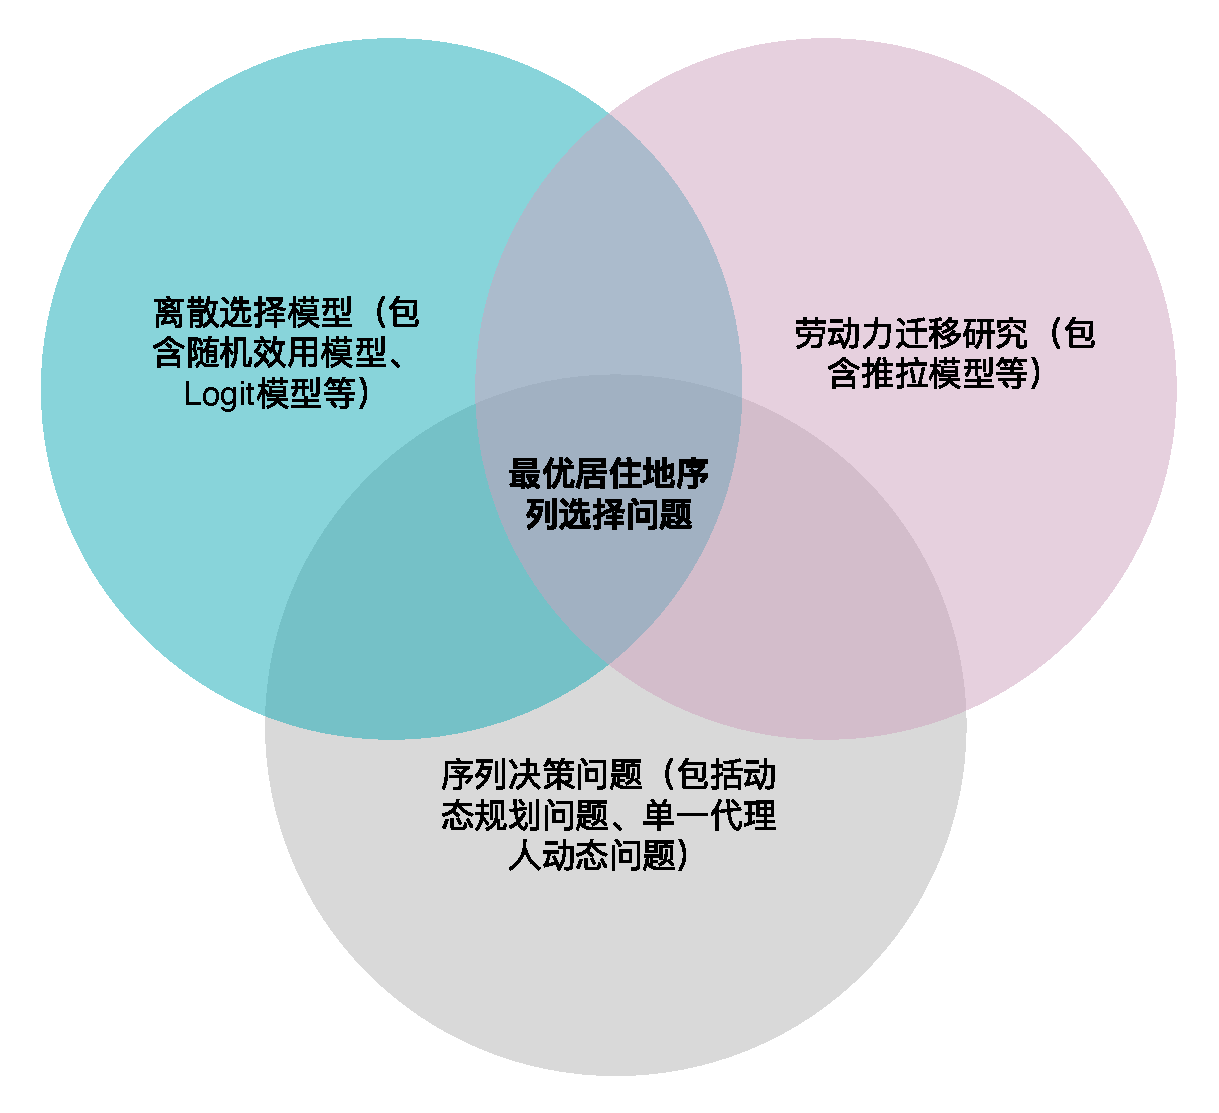
\includegraphics[width=0.8\textwidth]{images/optimal_residential_sequence.drawio.pdf}
\label{fig:最优居住地序列选择问题的理论来源venn diagram}
\end{figure}
























% ---------------------------------------- 理论模型 ----------------------------------------
\chapter{理论模型}

劳动力流动问题本质上极为复杂。经过前述分析,我们认识到,劳动力流动和迁移不应被简单地视为一次性经济活动,而应被理解为贯穿个体整个生命周期的持续决策过程。个体有在多个地理位置之间自主选择的自由意志,每个位置均对应一种独特且互斥的收益流(payoff flow)。当个体\footnote{本文中出现的个体指可以独立做出决策的经济单位,其具体形式可能为个人,也可能为家庭。为了消除歧义,后文将尽可能使用“决策者”一词代替。}做出迁移决策后将承担相应的迁移成本。决策者在不同阶段根据自身状况和外部环境变化,不断权衡是否迁移、迁移到何处,以及迁移后如何实现自身利益最大化。

本文通过动态离散选择框架构建了迁移序列动态决策模型,其建模必要性源于三重内生性挑战:首先,传统静态模型无法捕捉生命周期中人力资本积累引致的迁移倾向时变特征;其次,观测数据中存在不可观测的个体异质性(如风险偏好、信息处理能力)与迁移决策互为因果;第三,区位间收益流具有时变协整性,需构建跨期关联约束下的预期效用函数。为此,本研究提出动态迁移决策模型(Dynamic Migration Decision Model, DMDM)。

\section{初步模型}

考虑一个封闭经济体,
人口流动仅发生在经济体内部,不存在国际移民或与外部世界的人口交换。
人口在各地区之间分布不均,且随时间动态变化。
假设人口的总量保持不变。
经济体由 $m$ 个离散地区组成,形成迁移网络$\mathcal{C} = \{1,2,\dots,m\}$,即个体决策者的居住地选择集。
各区域拥有固定的地理边界和空间关系,每个地区连通且可达,迁移连通性由$m$行$m$列的邻接矩阵$Adj=[j_{xy}\in\{0,1\}]$刻画。
不同的区域都具有独特的地区特征,这包括经济特征与非经济特征等,每个地区的特征会影响个体的迁移决策。
各地区的工资由本地劳动力市场决定。
时间被划分为离散的时期$t=\{0,1,2,\ldots,t,t+1,\ldots\}$。决策者获取效用,在每个时期以效用最大化为目标做出迁移决策。地区特征(如工资、就业机会)、经济状况和政策随时间变化,影响个体的预期和决策。

同时经济体中实施户籍制度。
令居民的出生地为其户口所在地$hukou$。
如果决策者的户口所在地与其当前所在不同,就会对其福利、基础设施的获取造成负面影响,从而降低效用的获取。反之,则会增加效用。户籍制度对于决策者的影响效果如图\ref{fig:户籍制度造成影响的途径}所示。
\footnote{
这样的经济体会产生迁移吗?
在劳动力自由流动的经济体中,地区间收入差异会因劳动力迁移而趋于收敛,但非经济因素的地区差异仍然存在。即使在非经济因素趋同的特殊情形下,由于决策者的地区偏好设定,劳动力流动仍将持续存在。此外,本文还引入了户籍制度障碍、家乡溢价和迁移成本,进一步制约了劳动力的自由流动,降低了地区收入差异收敛的能力。
}

\begin{figure}[!ht]
\centering
\caption{户籍制度造成影响的途径}
\label{fig:户籍制度造成影响的途径}
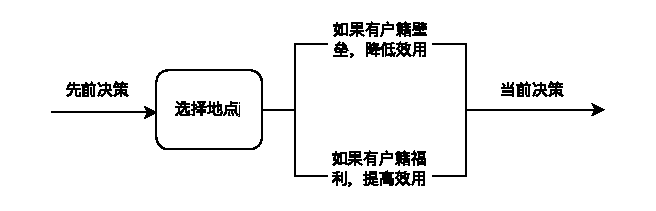
\includegraphics[width=0.8\textwidth]{images/户口影响.drawio.pdf}
\end{figure}


假设资产不影响居民的选择,考虑一个理性的决策者在$T$期生命周期内选择最优居住地序列。令$j_t \in \mathcal{C}$表示第$t$期的居住地选择,那么完整的选择序列可表示为$\mathcal{J}=\{j_1, j_2 ,\dots,j_T\}$。典型的居住地选择模式如表格\ref{tab:居住地选择序列可能的形式}所示。

\begin{table}[!ht]
\centering
\begin{tabular}{@{}ll@{}}
\hline
\multicolumn{1}{c}{\textbf{个体流动形式}} & \multicolumn{1}{c}{\textbf{居住地选择序列}}    \\ \midrule
\begin{tabular}[c]{@{}l@{}}\textbf{长期定居}:决策者在特定时间段内总是\\ 停留在同一个地区\end{tabular}                          & $\mathcal{J}=\{\dots, 1,1,1,1,1,\dots\}$ \\
\begin{tabular}[c]{@{}l@{}}\textbf{单向迁移}:如果 $j_p \neq j_q, \forall p\neq q$,那么\\ 个体就进行了迁移\end{tabular} & $\mathcal{J}=\{\dots, 1,2,3,4,5,\dots\}$ \\ 
\textbf{回流迁移}:返回到先前居住过的地区                      & $\mathcal{J}=\{\dots, 1,2,2,1,1,\dots\}$ \\ \bottomrule
\end{tabular}
\caption{居住地选择序列可能的形式}
\label{tab:居住地选择序列可能的形式}
\end{table}


决策问题由状态变量$x_t$刻画,其包含
个体特征(年龄、收入、家庭规模等)、
地区属性(房价、公共设施等)、
历史居住选择记录、
宏观经济环境
等因素。
状态转移服从马尔可夫过程,其转移概率为$p(x_{t+1}|x_t,j_t)$。

决策者在第$t$期从居住地$j$
\footnote{本文中$j$代表可选择的地点,而$j_t$代表个体在$t$期做出的具体选择。}
获得的地区效用为:
\begin{equation}
  \tilde{u}_t(j, x_t) = u_t(j, x_t)  +  \zeta_{jt}
  \label{eq:地区效用函数}
\end{equation}
其中$u_t(j, x_t)$为确定性效用项,
$\zeta_{jt}$为在任意时期和地点都独立同分布的随机扰动项,服从标准Gumbel分布$F(\zeta) = \exp(-\exp(-\zeta))$,且与状态变量$x_t$无关。


理性决策者做出选择的标准是选择使得效用最大化的选项:
\begin{equation}
  j_{it} = \arg\max_{j \in C} \{\tilde{u}_t(j, x_t)\}
\end{equation}

对于在选择集$\mathcal{C}$中选择$j$的概率可以写为:
\begin{equation}
\begin{split}
  Pr(\text{选择地点j})&=Pr(\tilde u_j > \tilde u_k, \forall k \neq j)
  \\&=Pr(u_j+\zeta_j>u_k+\zeta_k, \forall k \neq j)
  \\&=Pr(\zeta_k-\zeta_j<u_j-u_k, \forall k \neq j)
\end{split}
\label{eq:C中地点选择j的概率}
\end{equation}

在动态框架下,决策者具有前瞻性,并且通过最大化期望折现效用进行跨期优化。决策者在每期进行最优的居住地选择,或者说决策者选择$T$维的最优居住地选择序列$\mathcal{J}^*=\{j_1^*,j_2^*,\ldots,j_T^*\}$。每期的效用可以分为两部分,一是选择地点$j \in \mathcal{C}$带来的当期效用,二是折现的通过转移概率加权得到的未来期望效用。

假设折现因子为$\beta \in (0,1)$,决策者的目标是为从$t$期开始的期望折现效用最大值,这可以表示为:
\begin{equation}
  V_t(x_t, \zeta_{j_t}) = \max_{j_t \in \mathcal{C}} 
  \left\{ 
  \tilde{u}(j_t, x_t) + \beta \sum_{x_{t+1}} p(x_{t+1} | x_t, j_t) \cdot \mathbb{E}_{\zeta_{j_{t+1}}} [ V_{t+1}(x_{t+1}, \zeta_{j_{t+1}}) ]
  \right\}
\end{equation}
其中$\mathbb{E}_{\zeta_{j+1}} v_{t+1}(x_{t+1},\zeta_{j+1})$
为在状态 
$x_{t+1}$下,对所有可能随机扰动 
$\zeta$取期望后的长期效用。

那么决策者的基本问题就是在每个给定状态$x$和随机项 $\zeta_j$的情况下,选择最优居住序列$\mathcal{J}^*$使得全生命周期中的期望折现效用最大化,即:
\begin{equation}
  \max_{\mathcal{J}=\{j_1,j_2,\ldots,j_T\}} \mathbb{E} [ \sum_{t=1}^{T} \beta^{t-1} \tilde{u}_{j_t}(j_t,x_t) ]
\end{equation}

也可以使用迭代形式,即决策者每期都选择$j$来实现使得个体在生命周期中的总效用最大化,
令
$\begin{cases}
  v(j_{t},x_{t})=u(j_{t} ,x_{t})+\beta \sum_{x_{t+1}} p(x_{t+1}|j_t,x_t) \cdot \mathbb{E}_{\zeta_{j+1}} V_{t+1}(x_{t+1},\zeta_{j+1})
  \\
  \bar v(x_{t})=\mathbb{E}_{\zeta_{j_t}} v_{t}(x_{t},\zeta_{j})
\end{cases}$
,其中$E_{\zeta}$表示对 J 维向量$\zeta$的分布求期望\footnote{对于决策者而言收益冲击$\zeta$在做出居住地选择决策之前就已经实现,而$v(x,j)$ 和 $\bar v(x)$ 之间的区别在于,一个表示每个替代选择的延续值,而另一个表示在收益冲击实现之前所取的优化延续值的期望。},决策者基本问题的迭代形式为:
\begin{equation}
V(x,\zeta)=\max\limits_{j}[v(j,x)+\zeta_{j}]
\end{equation}

图片\ref{fig:migration_flow_resized2} 展示了一个动态规划决策过程。在离散周期$t$结束时或者下个周期$t+1$即将开始时,决策者根据在抽取到的随机收益冲击$\zeta$和状态转移概率$p(x_{t+1}|x_t,j_t)$双重不确定性的影响下通过Bellman方程做出决策,进入下一个周期$t+1$后获得该期的效用$\tilde u_{t+1}$。

\begin{figure}[!ht]
\centering
\caption{动态离散选择模型下的劳动力迁移决策流程图}
\label{fig:migration_flow_resized2}
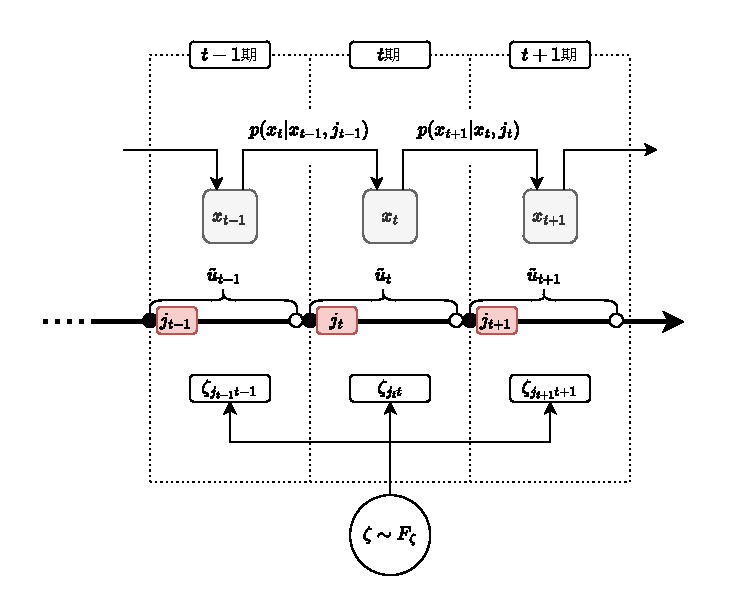
\includegraphics[width=0.9\textwidth]{images/dynamicsequence2.drawio.pdf}
\end{figure}

由于随机效用项$\zeta_j$独立同分布且服从 I 型极值分布,根据\cite{mcfaddenConditionalLogitAnalysis1973,rustOptimalReplacementGMC1987,rustStructuralEstimationMarkov1994}的结论,可知:
\begin{equation}
  \exp(\bar v(x_t))=\sum\limits_{k=1}^{J}\exp(v(x_t,k_t))
\end{equation}
可知选择地点j的概率,即公式\ref{eq:C中地点选择j的概率},存在softmax函数形式,这是由Gumbel噪声的极值分布性质推导的:
\begin{align}
\rho(x,j)&=\exp(v(x,j)-\bar v(x))
\\&=\frac{\exp(v(x,j))}{\sum\limits_{k\in J} \exp(v(x,k))} \label{eq:地点选择概率}
\end{align}
这极大地优化了动态规划问题中期望值的计算,并且由于sotfmax函数输出的概率分布是平滑的,有利于策略迭代的稳定性。


%由于随机效用项$\zeta_j$独立同分布且服从 I 型极值分布,其概率累积分布为$F(\zeta_j)=\exp(-\exp(-\zeta_j+\bar \gamma))$,其中$\bar \gamma$为欧拉常数。

%$\max_j \left(v(x,j)+\zeta_j\right)$的期望为$\bar v(x) = E_\zeta V(x,\zeta)= \ln(\sum\limits_{k=1}^J \exp(v(x,k)))+\bar \gamma$。这表明$\exp(\bar v(x)-\bar \gamma)=\sum\limits_{k=1}^J \exp(v(x,k))$。将其简化为,$\exp(\bar v(x))=\sum\limits_{k=1}^J \exp(v(x,k))$。

%利用Gumbel分布的封闭性质,将选择地点$j$的概率事件表达式化为$\rho(x,j)=\exp(\bar \gamma + v(x,j) - \bar v(x))$,
%将$\bar v(x)$的定义式代入其中,化简后利用指数运算的特性可得动态离散选择中的地点选择概率\footnote{这实际上也是softmax函数的一种概率向量形式,可以在动态模型中通过$\bar v(x) = \ln (\sum \exp(v(x,k)))+\bar \gamma $将未来效用递归嵌入当前选择。}
%\begin{equation}
%  \rho(x,j)=\frac{\exp(v(x,j))}{\sum\limits_{k=1}^J \exp(v(x,k))}
%\end{equation}


\section{效用函数具体构成}

接下来为公式\ref{eq:地区效用函数}赋予具体形式,从而使其具有经济意义。
假设个体决策者$i \in \mathcal{N}$的
家乡为$h$,那么该点上可能的效用流为:
\begin{equation}
  \tilde u_{t}^h(j_t,x_t;\theta)=u_{t}^h(j_t,x_t;\theta) +\zeta_{j_t,t}
  \label{eq:家乡效用函数}
\end{equation}

假设收入的边际效用是固定的,居民可以在固定利率下自由借贷,那么居民的期望效用最大化问题就可以转化为预期永久收入\footnote{永久收入以现值形式记录。}
减去一次性付清的迁移成本。
\footnote{
假设效用函数的线性形式为$U(x)=a X$,其中a为边际效用参数。居民可在固定利率$r$下无限制借贷,预算约束满足消费现值等于收入现值。
居民可以留在原地(永久收入为$Y_h$)或迁移(永久收入为$Y_p$,后者需支付一次性迁移成本 $M$。
假设迁移成本 
$M$
为即期支出,且永久收入为永续年金。

若居民留在原地,其永久收入的现值为
$W_h = \sum\limits_{t=0}^\infty \frac{Y_h}{(1+r)^t}=\frac{Y_h}{r}$,
总效用为$U_h=a W_h = \frac{a Y_h}{r}$。
若居民选择迁移,需支付即期成本 
$M$
,迁移后的永久收入现值为
$W_h = \sum\limits_{t=0}^\infty \frac{Y_p}{(1+r)^t}=\frac{Y_p}{r}$,
由于迁移成本 
$M$
为即期支出,净现值为
$\mathcal{W}=W_p-M=\frac{Y_p}{r}-M$,
总效用为
$U_p=a(\frac{Y_p}{r}-M)$
迁移的条件为$U_p>U_h \Rightarrow a(\frac{Y_p}{r}-M) > a \frac{ Y_h}{r} \Rightarrow Y_p-Y_h > rM$。
期望效用最大化等价于选择净现值更高的选项,即$\max\{a(\frac{Y_p}{r}-M), a \frac{ Y_h}{r}\}$。
}
居民的基础效用由货币性收入、城市宜居度、家乡溢价减去迁移成本组成。令效用函数为如下形式:
\begin{equation}
  \begin{split}
    u_t^h(j_t,x_t;\theta)=&\alpha_0 \cdot w_{ijt}+\sum\limits_{s} \alpha_{s} \cdot y_{s}(j_t)  + \alpha_h \cdot I(j_t=h) 
    \\& + \alpha^p \cdot I(j_t \neq hukou) +\xi(j_t,\omega)-\kappa(j_t,j_{t-1},x_t)
  \end{split}
  \label{eq:家乡效用函数中的具体构成}
\end{equation}
其中$\theta$代表参数向量, $w(j_t,\omega_t)$为经济收益函数,衡量个体在当前位置通过劳动获得的经济收益,$\alpha_0$表示工资收入对效用的权重(边际效用);
$y_{s}(j_t)$为该居住地提供的非货币性舒适度(amenity)价值,如气候、公共服务、文化等,反映地理位置的非经济吸引力,$y_s$是第$s$种舒适度的量化指标(如教育质量指数),其边际效用由$\alpha_s$表示;
$\alpha_h \cdot I(j_t=h)$是对家乡的偏好溢价,$\alpha_h$衡量个体对出生地的情感依恋强度,其中$I(\cdot)$为指示性函数,当其中判断为真时返回1,否则为0,这意味着只有当当前所在地是家乡时效用才会额外增加$\alpha_h$;
$\alpha^p \cdot I(j_t = hukou)$为人户分离时的制度障碍效应,只有当所在地与户籍地不同时才会产生$\alpha^p$单位的效用增减;
$\xi(j_t,\omega)$为个体的地区偏好成分,
反映个体对某地点的长期偏好匹配(如文化契合度),仅当个体访问该地点时才能获知其具体值;
$-\kappa$为从其他区域前往地区$j$的迁移成本函数,负号表示迁移成本会降低效用,包括直接费用(如搬家费)和间接成本(如适应新环境的心理成本)。



公式\ref{eq:家乡效用函数中的具体构成}中,决策者的经济收益函数由多种因素组成。在不考虑时间因素的影响下,个体决策者$i \in \mathcal{N}$在地区$j \in \mathcal{C}$的收入设定为以下函数形式:
\begin{equation}
  w_{ij}=\mu_j + \nu_{ij} + G(X_i,a,t) + \eta_i + \varepsilon_{ij}(a)
  \label{eq:经济收益函数}
\end{equation}
地区基准收入$\mu_j$反映地区$j$的平均工资水平,
代表地区的经济基本面,如生活成本、区域产业聚集效应(如北京的传媒业、山西的采矿业)、政策红利(税收减免、人才补贴)等结构性特征,是所有在该地点个体的工资基准,
其与个体无关,仅取决于地点特征。
个体-地区匹配效应$\nu_{ij}$表征相同技能劳动者在不同地区的收入差异,
捕捉个体与地区的特殊适配性(如技能需求匹配、文化契合度),例如,程序员在科技中心可能获得更高的$\nu_{ij}$,
其具备匹配效应在个体驻留期间保持稳定,一旦个体进入地区 $j$,
$\nu_{ij}$固定不变,但迁移到新地区$k$ 时会生成新的 $\nu_{ik}$\footnote{在这点上与地区偏好$\xi$类似,但前者可通过工资和迁移选择共同推断,而后者仅能通过迁移选择推断。}。
匹配效应实现值$\nu_{ij} \sim F_\nu$在个体进入地区$j$后方可观测。
生命周期收入$G(X_i,a,t)$为线性函数,其包含三重要素,
个体特征$X_i$包含教育程度、性别等,
年龄效应$a$反映人力资本积累曲线,
时间趋势$t$捕捉技术进步等外生冲击。
量化系统性因素对工资的影响(如工作经验随年龄增长、宏观经济波动)。
$G$ 的影响在不同地区间相同(如教育回报无地区差异)。
个体固定效应$\eta_i$表征表示个体 $i$ 异质性中不随地区改变的固有能力或特质,
如先天能力、家庭背景等,无论迁移到哪里均保持恒定。
假设个体已知 $\eta_i$ 的值,并在决策中利用此信息。
暂时性随机效应$\varepsilon_{ij}(a)$代表短期波动或随机扰动项,服从i.i.d分布的当期扰动,
捕捉不可预测的工资波动(如临时绩效波动、经济冲击)。
假设$\varepsilon$服从期望为0的正态分布,并且独立于其他变量,随年龄和时间变化,个体无法预知其实现值\footnote{所以即使暂态效应对于每个地点都不同,但对居住地选择决策无持续影响。}。

如果发生了迁移($j_t \neq j_{t-1}$),同个决策者$i$的迁移成本$\kappa$设定为以下函数形式:
\begin{equation}
\begin{split}
  \kappa=I(j_t \neq j_{t-1}) \cdot [& 
  \gamma_{0 \tau}
  + \gamma_1 D(j_{t-1},j_t)
  - \gamma_2 I(j_t \in Adj(j_{t-1}))
  \\&
  - \gamma_3 I(j_t \in Pre)
  + \gamma_4 a
  -\gamma_5 n_j
  ]
\end{split}
\label{eq:迁移成本函数}
\end{equation}
$\gamma_{0\tau}$迁移中类型相关的的固定成本,随个体类型 $\tau$ 变化,从而捕捉未观测的异质性。例如:  
“定居型”个体(stayer type)的 $\gamma_{0\tau}$ 极高,几乎禁止迁移;
“流动型”个体的 $\gamma_{0\tau}$ 较低,更易迁移。不同类型的群体分布由对应的概率$\pi_\tau$给出,并且满足$\sum\limits_{\tau}^{} \pi_\tau=1$。
$\gamma_1 D(\ell^0, j)$为迁移距离效应,是 $D(\ell^0, j)$ 的线性成本(以大圆距离衡量),距离越远,成本越高($\gamma_1 > 0$)。  
$-\gamma_2 \chi(j \in A(\ell^0))$是相邻地区效应,若目标地点 $j$ 与当前地点 $\ell^0$ 相邻(即 $j \in A(\ell^0)$),则成本减少 $\gamma_2$。
相邻地区迁移可能因文化相似、信息透明或交通便利而成本更低($\gamma_2 > 0$)。  
$-\gamma_3 \chi(j = \ell^{-1})$为历史地区效应(回流效应),
其定义为若目标地点 $j$ 是个体曾居住过的历史地点 $\ell^{-1}$,则成本减少 $\gamma_3$。
这是因为返回熟悉地区可能因现存社会网络或无需重新适应而成本更低($\gamma_3 > 0$)。  
$+\gamma_4 a$代表年龄障碍效应,表明迁移成本随年龄 $a$ 线性增加,年龄越大,迁移的心理或生理成本越高($\gamma_4 > 0$)。  
$-\gamma_5 n_j$为目标地区规模成本效应,
目标地区人口规模 $n_j$ 越大,迁移成本减少 $\gamma_5 n_j$。  
这是因为
大规模地区可能有更多潜在支持(如亲友网络、服务机构),减少安家难度,从而降低迁移成本($\gamma_5 > 0$),符合“引力模型”中人口规模吸引迁移的经典结论。  
$I(j_t \neq j_{t-1})$为迁移指示函数 ,仅当目标地点 $j \neq \ell^0$ 时,迁移成本生效(否则为0)。  这确保个体留在原地时无需支付迁移成本。

迁移成本中参数的经济含义如表格\ref{tab:迁移成本参数释义}所展示。
\begin{table}[!ht]
  \centering
  \caption{迁移成本参数释义}
  \label{tab:迁移成本参数释义}
  \begin{tabularx}{\textwidth}{@{}llX@{}}
    \toprule
    \multicolumn{1}{c}{\textbf{参数符号}} & \multicolumn{1}{c}{\textbf{参数含义}} & \multicolumn{1}{c}{\textbf{参数意义}} \\ \midrule
    \multicolumn{1}{c}{$\gamma_{0\tau}$} & 类型异质效应 & 捕捉不同类型的异质性,可以解释为何有些人从不迁移,识别“定居型”人群可针对性地设计激励措施(如搬迁补贴)。\\ 
    \multicolumn{1}{c}{$\gamma_1$} & 物理迁移成本 & 个体与其携带物必然因为物理法则而产生运输成本。 \\ 
    \multicolumn{1}{c}{$\gamma_2$} & 相邻地区效应 & 反映地理邻近性的普遍优势。 \\ 
    \multicolumn{1}{c}{$\gamma_3$} & 历史地区效应 & 返回历史地区因熟悉度获得折扣,体现路径依赖。 \\ 
    \multicolumn{1}{c}{$\gamma_4$} & 年龄障碍效应 & 针对不同年龄群体制定差异化迁移政策(如青年人才引进计划)。\\ 
    \multicolumn{1}{c}{$\gamma_5$} & 规模成本效应 & 大地区吸引力不仅体现在经济机会(如工资 $\mu_j$),也直接降低迁移成本。\\ \bottomrule
  \end{tabularx}
\end{table}


此外,由于暂态效应$\varepsilon$服从期望为0、标准差差为\(\varepsilon_{it}\)的正态分布,已知经济收益函数设定为公式\ref{eq:经济收益函数}。
令$\phi$表示标准正态分布的概率密度函数,处于地点$j$的个体$i$在时期$t$的经济收益函数的密度函数$\Psi_{it}$为:
\begin{equation}
  \Psi_{it}=\phi(\frac{w_{it} - \mu_{jt} - G_{it} - \nu_{ijt} - \eta_i }{\sigma_{\varepsilon_{it}}})
  \label{eq:经济收益似然贡献}
\end{equation}
这在实际上是决策者的似然贡献之一。

\section{状态转移概率}

本文将决策者在不同时期的迁移决策组成一个序列,并将其建模成一个马尔可夫决策过程(Markov Decision Process, MDP)。
MDP包括两个核心假设决策具有目标性和Markov性。决策的目标性 指个体在每个状态下选择一个行动,目标是最大化某种累积奖励(长期收益)。
状态转移的 Markov 性 指下一时刻的状态仅依赖于当前状态和采取的行动,而与过去的状态和行动无关
\footnote{在许多实际场景中,个体的迁移决策确实主要基于当前的状态(如当前所在城市的生活成本、就业机会、家庭因素等),而不是过去的迁移历史。因此,本文的Markov 性假设是合理的。}。
状态变量转移概率描述的是在选择了特定位置$j_{t}$的情况下,从状态 $x_t$ 移动到新状态 $x_{t+1}$的条件可能性。
本文假设状态变量转移概率具有马尔可夫性
,即系统的未来状态仅依赖于当前状态和当前决策,与过去的历史无关,这意味着:
\begin{equation}
  p(x_{t+1}|x_{t},j_{t},x_{t-1},j_{t-1},\ldots)=p(x_{t+1}|x_{t},j_{t})
\end{equation}
该假设,符合沉没成本理论,大大简化了问题的复杂度。

根据先前的模型假设,决策者只有在迁移到某个地点时才能了解真实的工资和效用匹配值,因此新的目的地是随机抽取新的匹配值的。
具体而言,本文将其设置为:
\begin{equation}
  p(x_{t+1}|x_t,j_t)=
  \begin{cases}
    % 迁移
    \frac{1}{m^\omega}
    , &\text{发生迁移从而产生随机抽取}
    \\
    % 不迁移
    1
    , &\text{没有迁移}
    \\
    % 其他
    0
    , &\text{其他情况}
  \end{cases}
\end{equation}


将状态变量 \( x \) 分解,实际为包含一个 \( M \) 维的最近位置向量 \( \ell \)、一个 \( m \) 维的与位置相关的工资和效用信息向量 \( \omega \),以及个人年龄 \( a \)。为了计算简便,状态向量定义为 \( x = (\tilde{x}, a) \),其中 \( \tilde{x} = (l^0, l^1, x_0^0, x_0^1, x_\xi^0, x_\xi^1) \)。其中,\( l^0 \) 表示当前位置 \( j_t \),\( l^1 \) 表示上一个位置 \( j_{t-1} \)。索引 \( x_0^0 \) 和 \( x_0^1 \) 分别对应于当前和先前位置的工资匹配值 (\( v_{i l^0} \), \( v_{i l^1} \)),而 \( x_\xi^0 \) 和 \( x_\xi^1 \) 则表示效用匹配值 (\( \xi_{l^0} \), \( \xi_{l^1} \))。年龄 \( a \) 捕捉了个体状态的时间维度。

1. 无迁移 (\( j_{t+1} = j_t \)):如果个体停留在当前位置 (\( j_{t+1} = l^0 \)),状态分量保持不变 (\( \tilde{x}' = \tilde{x} \)),年龄增加 1 (\( a' = a + 1 \))。转移概率为 1,反映工资和效用匹配 (\( v_{i l^0} \), \( \xi_{l^0} \)) 保持不变。

2. 返回先前位置 (\( j_{t+1} = j_{t-1} \)):当个体返回先前位置 (\( j_{t+1} = l^1 \)) 时,当前位置和先前位置互换 (\( l'^0 = l^1 \), \( l'^1 = l^0 \))。工资和效用匹配指数会相应更新:先前位置的工资指数变为当前工资指数 (\( x_0'^0 = x_0^1 \)),当前位置的工资指数变为先前工资指数 (\( x_0'^1 = x_0^0 \))。同样,效用指数也会互换 (\( x_\xi'^0 = x_\xi^1 \), \( x_\xi'^1 = x_\xi^0 \))。年龄递增 (\( a' = a + 1 \)),转移概率为 1。这保留了历史匹配信息,反映了路径依赖性,而无需重新抽取。

3. 迁移到新位置 (\( j_{t+1} \notin \{ j_t, j_{t-1} \} \)):如果个体移动到新位置 (\( j_{t+1} = j \)),则当前位置更新 (\( l'^0 = j \)),并且先前位置变为之前的当前位置 (\( l'^1 = l^0 \))。新的工资和效用匹配分别从具有 \( n_0 \) 和 \( n_\xi \) 个可能值的离散分布中随机抽取,索引分别为 \( s_0 \in \{1, \dots, n_0\} \) 和 \( s_\xi \in \{1, \dots, n_\xi\} \)。因此,\( x_0'^0 = s_0 \) 和 \( x_\xi'^0 = s_\xi \),同时保留先前位置的匹配 (\( x_0'^1 = x_0^0 \)、\( x_\xi'^1 = x_\xi^0 \))。年龄递增 (\( a' = a + 1 \)),转移概率为 \( \frac{1}{n^2} \)(假设 \( n_0 = n_\xi = n \)),反映了对新地点匹配的独立且均匀的抽取。

4. 无效转移:上述情况未涵盖的任何转移的概率为 0,以确保仅考虑有效的地点选择。

并且,该设置通过索引匹配值而不是存储其显式值,从而压缩状态空间,以利于求解数值。
转移概率反映了决策者对新地点的探索,其中工资和效用信息仅在抵达时才会显示,而历史数据则会保留以备潜在的返回迁移。这种结构支持在信息不完整的情况下进行动态决策,平衡对新位置的探索和对已知路径相关信息的依赖。

\section{劳动力迁移决策}

由于地区偏好效应和个体固定效应仅与个体特征相关,而暂态效应仅在迁移至目的地后随机产生,因此这两个因素不会影响决策者的迁移选择。
在不同地区$j$和$k$之间,仅有平均工资$\mu$、地区匹配效应$\nu$和非经济因素存在地区间差异。
地区选择通过影响收入水平而产生作用,劳动力将倾向于选择具有更优劳动力市场条件、更高地区匹配效应和更高宜居度条件的目的地。
然而,这种选择必须同时满足预期收益需超过户籍制度障碍、迁移成本、心理成本(如恋家效应)以及随机效用冲击等因素造成的阻力。
简言之,外部条件对决策者效用的提升必须足以克服迁移过程中的各类障碍,这恰如公式\ref{eq:迁移motivation}所示。
\begin{equation}
\begin{split}
  Pr(\text{选择k})&= Pr(u_k - u_j > \zeta_j - \zeta_k) 
  \\&= Pr(
  \text{地区k的客观因素} - \text{地区j的客观因素} 
  > 
  \underbrace{\alpha^p}_{\text{制度}} + \underbrace{\alpha^h}_{\text{心理}} + \underbrace{\kappa}_{\text{迁移成本}} + \underbrace{
  \zeta_j - \zeta_k}_{\text{外生冲击}} 
  )
  \\&= p >0
\end{split}
\label{eq:迁移motivation}
\end{equation}

至此,模型刻画出了在有限生命周期内,每期决策者可以在迁移网络$\mathcal{C}$中自由选择最优住址$j_t$,这些不同时期的选择构建出了最优居住地选择序列$\mathcal{J}$。这意味着迁移可以是多次的,可撤回的。




% ---------------------------------------- 实证部分 ----------------------------------------
\chapter{实证处理}

\section{模型上} 

采取动态规划方法的一个缺陷在于计算上很容易陷入维度的诅咒(curse of dimensionality),出于实证处理的简便处理,本文将对于模型中一些难以计算的点进行简便假设。

\subsection{年龄效应}
出于简化
参照以往的计量经济学经验
将年龄效应设置为年龄的有待估参数的一次项和二次项的和
\ref{eq:家乡效用函数中的具体构成}中的$G$设置为
$$G=r_1 a + r_2 a^2$$


\subsection{非参数离散混合方法} 

基于上述模型设定,公式\ref{eq:家乡效用函数中的具体构成}中的地区偏好$\xi$、公式\ref{eq:经济收益函数}中的个体固定效应$\eta$、地区匹配效应$\nu$以及暂态效应$\varepsilon$的具体函数形式仍未确定。若无法解决这一识别问题,将难以准确计算决策者的效用函数和期望值。因此,有必要对这些随机项的概率分布施加合理的假设和约束条件。

出于计算上的简便,
本文使用支撑点离散化方法。
对于任何不知道其分布的 $F$,我们可以找到最佳近似分布 $\hat F$ 来近似。对于连续分布的变量$F$,离散的 $\hat F$ 是一组有限的支撑点组成,每个支撑点都有对应的概率值,即$\{(x_i, p_i)\}, 1 \leqslant i \leqslant N$ 的组合,其中 $x_i$ 是离散点,$p_i$ 是其概率,$N$ 为给定的支持点数。
对于每个$q_r, (1\leqslant r \leqslant n )$,计算对应的效用值,用这些有限的效用值来代替连续效用的积分。
通过该处理后,模型变为有限状态的动态规划问题,可以直接构建似然函数并进行最大似然估计。
相较于蒙特卡洛模拟,该方法可以避免随机噪声,适合精确的极大似然估计。

由于假设分布围绕 0 对称,因此仅需要 $\frac{M-1}{2}$ 个支持点即可进行估计。

令 $p_i = \frac{1}{N}, \forall i$。


对于$\nu$
在每个地点中个体都有从地区匹配效应的分布中抽取一个值,假设这个分布是一个有限集合上的均匀分布,$Y=\{\nu(1),\nu(2)...\nu(n_{\nu})\}$
其结果是$\omega^{i}_{\nu}$,$\omega^{i}_{\nu}(j)$代表在地点j的匹配效应,$1\leqslant j\leqslant N_i$,$N_i$是$i$到达过的地方的数量
总共有$\{\omega^{i}_{\nu}(1),\omega^{i}_{\nu}(2)...\omega^{i}_{\nu}(j)...\omega^{i}_{\nu}(N_i)\}$

$\xi$
地区匹配偏好也是如此
来自于$\Xi=\{\xi(1),\xi(2)...\xi(n_{\xi})\}$
其结果是$\omega^{i}_{\xi}$

$\eta$ 表示每个个体工资的固定成分(例如长期能力或个体特质)。
假设其分布是一个对称的离散分布,具有7个支持点。每个支持点有相等的权重。
因为是离散分布,只需要估计 3个参数:分布的中间点(中心趋势)和离散范围。
固定效应代表长期的工资差异来源,例如教育水平、经验等。
选择离散分布是为了简化复杂的连续分布,同时通过支持点捕捉关键的分布特性(如中心趋势和差异性)。
$\eta$的离散分布提供了一种对长期工资特质的简化建模方式,减少计算复杂度,同时保留重要信息。
固定效应也是如此
来自于$H=\{\eta(1),\eta(2)...\eta(n_\eta)\}$
其结果是$\omega^{i}_{\eta}$


暂态效应$\varepsilon$在本质上是一种外生冲击,所以可以假设为服从期望为$0$的正态分布$N(0,\sigma^2)$,
保留了异方差特质以变容纳更多的异质性。
数学上$\varepsilon$表示工资的短期波动成分,比如由于经济周期、随机冲击等导致的变化
假设$\varepsilon_{it}$(某人在某个时间的短期波动)来源于一个均值为零的正态分布,其方差$\sigma_{\epsilon}$随人而异
对于每个人,$\sigma_\varepsilon(i)$来自一个离散分布(4 个支持点,均匀分布),因此需要估计 4 个参数
$\varepsilon$反映工资中不可预测的临时变化,例如经济不确定性或工作绩效波动
允许$\sigma_\varepsilon(i)$因人而异捕捉到工资短期波动的个体差异性(例如高风险行业可能有更大波动)
在建模中,$\varepsilon$允许方差随个体变化,体现了个体的异质性,这进一步增加模型的灵活性,使其能够更好地拟合数据。

暂态效应来自于一个期望为$0$的正态分布,但是假设其异方差使其可以可以容纳更多的异质性。
即$\varsigma=\{\sigma_{\epsilon}(1),\sigma_{\epsilon}(2)...\sigma_{\epsilon}(n_{\epsilon})\}$,
其结果是$\omega^{i}_{\epsilon}$。




表格\ref{tab:未观测到的变量表}总结了以上未知分布变量的设定。


\begin{table}[!ht]
\centering
\caption{未观测到的变量表}
\label{tab:未观测到的变量表}
\begin{tabular}{@{}ccccc@{}}
\toprule
变量 & 变量符号 & 分布假设 & 数量 & 抽取结果 \\ \midrule
地区匹配效应 & $\nu$ & $Y=\{\nu(1),\nu(2)\ldots\nu(n_{\nu})\}$ & n & $\omega^{i}_{\nu}(j)$\\
地区偏好 & $\xi$ & $\Xi=\{\xi(1),\xi(2)\ldots\xi(n_{\xi})\}$ & 1 & $\omega^{i}_{\xi}$ \\
固定效应 & $\eta$ & $H=\{\eta(1),\eta(2)\ldots\eta(n_\eta)\}$ & 1 & $\omega^{i}_{\eta}$ \\
暂态效应的方差 & $\varepsilon$ & $\varsigma=\{\sigma_{\varepsilon}(1),\sigma_{\varepsilon}(2)\ldots\sigma_{\varepsilon}(n_{\varepsilon})\}$ & 1 & $\omega^{i}_{\varepsilon}$ \\ \bottomrule
\end{tabular}
\end{table}


参数向量的可能实现组成一个集合,用$\Omega(N_{i})$表示,未观测到的因素组成一个$m_{i}+3$维的参数向量$\omega^{i}=(\omega^{i}_{\xi},\omega^{i}_{\eta},\omega^{i}_{\epsilon},\omega^{i}_{\nu}(1),\omega^{i}_{\nu}(2)...\omega^{i}_{\nu}(N_{i}))\in \Omega$。


对于公式\ref{eq:迁移成本函数}迁移成本函数中的异质性成本$\gamma_{0\tau}$,
模型假设随个体类型 $\tau$ 变化,从而捕捉未观测的异质性。
具体而言,本文将其分为分为3种类型。
类型1:高迁移倾向,低迁移成本,高不确定性容忍度。
类型2:中等迁移倾向,中等迁移成本,中等不确定性容忍度。
类型3:低迁移倾向,高迁移成本,低不确定性容忍度。
“定居型”个体(stayer type)的 $\gamma_{0\tau}$ 极高,几乎禁止迁移;
“流动型”个体的 $\gamma_{0\tau}$ 较低,更易迁移。
个体i属于类型k的概率为$\pi_k$,并且满足$\sum\limits_{k}^{} \pi_k = 1$。
每种类型的比例$\pi_1, \pi_2, \pi_3$作为模型参数被估计。
类型k的个体的效用函数为$u_{ijt}^k$,
模型可表示为:
$$V_{ijt}^k = u_{ijt}^k + \varepsilon_{ijt}^k + \beta^k E_t[V_{t+1}^k|d_{ijt}=1]$$
其中$k\in{1,2,3}$表示类型。


\section{似然函数}


由上文可知个体存在两种似然概率函数贡献,即公式\ref{eq:地点选择概率}和公式\ref{eq:经济收益似然贡献}。
通过个体在其历史轨迹中给出的两种似然贡献,
我们得到了类型为$\tau$的个体$i$的似然函数

即在所有可能的不可观测变量的组合下,个体在所有时期中的观测收入$w_{it}$上选择地点的概率$\rho_{it}$的乘积:
\begin{equation}
  L_{i}(\theta_{\tau})=\frac{1}{n_{\nu}n_{\epsilon}n_{\xi}(n_{\nu})^{N_{i}}} \sum\limits_{\omega^{i}\in\Omega(N_{i})}(\prod\limits_{i=1}^{T_{i}} \psi_{it}\lambda_{it})
\end{equation}

由于模型允许存在异质性

让$L_{i}(\theta_{\tau})$代表tau类型个体的似然函数,其中$\theta$是该个体的待估参数向量

样本的似然函数是一个混合类型的联合对数似然函数,把每个观测i的贡献相加
\begin{equation}
\Lambda(\theta)=\sum\limits_{i=1}^{N}\log(\sum\limits_{\tau=1}^{K}\pi_{\tau}L_{i}(\theta_{\tau})) 
\end{equation}
其中混合比例由$\pi_{\tau}$给出,且$\sum\limits_{\tau=1}^{K}\pi_{\tau}=1$
每个个体i都做出了贡献
这是在给定参数$\theta_{\tau}$的条件下,个体$i$在类型$\tau$下的似然。即,个体i可能属于某种类型,似然函数
$L_i(\theta_{\tau})$捕捉了该个体数据与类型$\tau$相关的匹配度。
混合似然$\sum_{\tau=1}^{K} \pi_{\tau} L_i(\theta_{\tau})$这表示对所有类型的加权平均,权重是$\pi_{\tau}$,即每种类型的概率。通过这种加权求和,模型允许每个个体属于不同的类型,并通过类型的权重(概率)来加权它们的贡献。

每个个体可能属于不同的类型,这些类型有不同的收入和行为模式。每个数据点i来自某个成分,但成分的归属是未知的,因此需要将每个数据点的似然表示为各成分似然的加权和,然后取对数并求和得到整个样本的对数似然。因此通过混合模型,能够捕捉到个体之间的异质性。


如此,通过最大似然计算,就可以得到各种参数的似然估计。

\section{迁移成本的似然函数}



% subsection 实证模型 (end)

\section{数据上}

地区数据的界限
由于劳动力的迁移在不同省之间呈现趋势 但在迁入大省中仍然存在人口净流出市 这说明劳动力移动的法律边界和现实边界存在重合 但是最好应该以市为标准 当然这一准则不包括某些政策带来的效应
上面说了为什么界限要往下卡在市,下面说一下为什么界限不继续往下到区或者村。首先是政策往往以市为最小执行单位;其次是在市内迁移中个人会为了出于固定资产投资等非模型考量的原因,这些原因并不是因为在迁居的地区能提供更好的个人预期工资
市级包含了县、乡、村等行政级别 每个市都包含了城市与农村(虽然城市化率略有不同)避免了城乡之间的划分对立


人口数据的界限
许召元2007

在我国存在广泛的农民工进城现象 大多数农民工只是暂时居住在


本研究使用CFPS2010年至2022年年两期数据构成面板进行影响评估。CFPS采用的是内隐分层、多阶段、多层次、与人口规模成比例的概率抽样方式,样本覆盖除中国港澳台、新疆、西藏、青海、内蒙古、宁夏和海南之外的其他省/市/自治区。这些地区的人口占全国的95\%左右,因此,CFPS的数据是一个具有全国代表性的高质量数据库。

\textit{关键结果变量为个人的年总收入 (PIncome)。本研究选取的关于个人总收入的变量为“qk601”(2010年) 和“p\_income”(2014 年) 。在面板数据中,两个变量统一命名为“PIncome”。该变量来自 CFPS 问卷的 “K 部分: 个人收入”,具体题目为“您 ( 去年)个人的年总收入是元?”。CFPS在公布历期数据之前,对收入部分结果进行了修正,以满足各年之间的可比性。控制变量。参考以往研究 (卜茂亮等,2011; 黄国英、谢宇,2017; 谭燕芝等, 2017; 周广肃、孙浦阳,2017) 并结合CFPS数据的可获得性和完整性,本文选取的控制变量包括地域 (所在省份)、常住地 (城镇或农村)、性别、民族、年龄、受教育年限、婚姻状态、自评健康状况、认知能力、非认知能力、对自己未来的自信心和职业等。其中CFPS的非认知能力来自访员在理解能力、配合程度、接人待物水平、回答的可信程度和语言表达能力5个方面对受访者的评价平均得分; 认知能力包括语文和数学方面的测试得分 (黄国英、谢宇,2017)}

本文选取2010年至2022年都存在记录的个体,

个体决策者的微观数据来源于自CFPS从2010年到2022年间的数据,
其记录了个人的迁移轨迹(将访问当年的地址视作居住地址)、年龄、收入等。


本文使用的地理数据包含我国31个省份(由于现行制度的不同和数据收集的难度,本文的数据排除了香港特别行政区、澳门特别行政区以及台湾省地区),
其中常住人口数量、人均可支配收入、自然灾害数据、城市人口数据、医疗数据、教育数据等数据来自于国家统计局公布的数据统计年鉴。


对于宜居度,本文将以下数据设为宜居度指标:

气候数据:
由于气候和空气质量在短期内发生变化的可能性较小,气候的对比不是局部发生变化的,以及气候数据在劳动力迁移决策中是用于进行横向对比而非纵向对比的,所以本文选用常量对每个省份的空气质量、日照时间、平均气温进行跨时间同一数值赋值。

气象:
\textit{PM2.5 浓度数据来源于 Van Donkelaar et al. ( 2016) 计算的全球年度 PM2. 5 卫星栅格数据。我们 首先利用地理信息系统将每个栅格定位到其空间位置所在的城市上,然后将落在每个城市内的所有 栅格数据进行平均,即可得到各个城市在不同年份的 PM2. 5 浓度水平。与地表监测的点源数据相比, 卫星观测数据在时间和空间上的覆盖范围更广,能够与我们的流动人口数据更好的匹配; 同时,卫星 监测数据相对更加客观和准确,能够避免很多人为因素导致的测量偏误( Ghanem \& Zhang,2014) 。}

最高温度平均数 最低温度平均数 紫外线强度 体感舒适天数  空气质量优良率



宜居度包括:
自然禀赋:
生活水资源


房价收入比:
本文选取房价收入比作为房价的宜居度表现形式。
房价数据来自于xxx。com网站

商业资源:
本文还使用各省每万人连锁餐饮门店数与每万人社会零售消费品总额(亿元)代表商业资源


本文的公共服务包含以下:

1.地方教育:
地方教育经费、地方医疗经费来自各省地方财政局网站公布的数据。
由于教育的变量存在高度相关性
所以使用主成分分析法将教育变量整合为一个指标

2.地方医疗:
同样的
对于医疗资源使用熵值法合成一个指标

3.市政设施:
城市用水普及率
城市燃气普及率
每万人拥有公共交通车数量
人均公园绿地面积(平方米/人)
每万人拥有公共厕所(座)
使用PCA主成分生成一个指标


对于省份的地理指标,本文将其进行如下处理:

距离数据各省市以其省会为,经纬度源自geopy的Nominatim,计算方法则基于其geodesic方法。
该方法基于WGS84椭球模型,考虑地球的扁率使得精度更高,使用Vincenty算法迭代计算两点间的最短测地线距离。
\footnote{
具体而言,
已知地球的
长半轴为$a = 6378137.0$ 米(WGS-84椭球的赤道半径),
扁率为$f = 1 / 298.257223563$,
则短半轴为$b = a(1 - f)$。
给定两点以弧度表示的经纬度坐标 $ P_1(\phi_1, \lambda_1) $ 和 $ P_2(\phi_2, \lambda_2) $,
计算经度差$\Delta\lambda = \lambda_2 - \lambda_1$,
再利用使用 Vincenty 公式求解两点之间的中心角 $\sigma$。
测地线距离 $d$ 的最终公式为$d = b \cdot A \cdot \sigma$,
其中$A$是与椭球扁率相关的修正系数。
}

在研究省份之间的迁移成本或区域经济联系时,地理邻接性是一个重要的影响因素。邻接省份通常具有更紧密的经济、文化和交通联系,这些因素会显著影响人口流动、资源配置以及区域协同发展。
邻接省份可能在区域性政策上更具一致性,这降低了迁移者的制度适应成本;邻接省份之间可能存在更紧密的经济联系,例如产业链上下游关系,为迁移者提供更多就业机会。
因此,为了量化省份之间的邻接关系,本文根据我国省级行政区划的地图信息,构建了一个邻接矩阵 A。
设 A 是一个 $N \times N$的方阵(其中 $N$ 为省份数量),每行和每列分别对应一个省份。对于矩阵中的任意元素 $a_{m,n}$而言,其对应的数值代表$m$省与$n$省之间的邻接关系,若邻接则取$1$,否则为$0$。
在构建邻接矩阵时,本文假设省份之间的邻接关系仅由地理边界决定,而不考虑其他因素(如交通网络密度或行政合作程度)。此外,受数据限制,本文暂不考虑海峡等自然障碍对邻接关系的影响。同样的,本文排除了港澳台三个地区。

中华人民共和国教育部发布的《中国语言文字概况(2021)》指出,我国有56个民族,是一个多民族、多语言、多方言、多文字的国家。普通话和规范汉字是国家通用语言文字,是中华民族通用的语言文字。
现代汉语有标准语和方言之分。
汉语方言通常分为十大方言:官话方言、晋方言、吴方言、闽方言、客家方言、粤方言、湘方言、赣方言、徽方言、平话土话。各方言区内又分布着若干次方言和许多种“土语”。其中使用人数最多的官话方言可分为东北官话、北京官话、冀鲁官话、胶辽官话、中原官话、兰银官话、江淮官话、西南官话八种次方言。
以往文献中速来有讨论方言对于劳动力流动的影响,
例如\cite{HuangZongYeFangYanDuiShengJiRenKouQianYiDeYingXiang2020,LiQinFangYanPuTongHuaYuZhongGuoLaoDongLiQuYuLiuDong2014}等,但是这些文献中往往将方言的影响局限于语言是否相同。
本文基于比较语言学中对于我国方言的大量研究,提出采用
基于树形结构的最近公共祖先(LCA)距离来划分各省市之间的方言亲近度。
\footnote{
对于一个有根树形结构$T=(V,E)$,其中
$V$表示树的顶点集合;
$E\subseteq V \times V$表示边的集合;
任意其中两个节点$u$和$v$,它们的最近公共祖先 $LCA(u,v) $定义为
$LCA(u,v)=\arg \max_{w\in V} depth(w)$,
其中 $w$ 是同时满足是 $u$ 和 $v$ 的祖先;$w$ 在树中的深度最大。
换句话说,$LCA(u,v)$ 是从根节点到 $u$ 和 $v$ 的路径上的最后一个公共节点。
}
公式\ref{eq:方言相似度}展示了对于各省代表性语言计算亲近度的方式。
\begin{equation}
  \label{eq:方言相似度}
  \text{方言相似度}=\frac{1}{1+\text{LCA depth}}
\end{equation}
本文使用的语言谱系树如图\ref{fig:linguistic_tree}所示。
\begin{figure}[!ht]
\centering
\caption{语言谱系树}
\label{fig:linguistic_tree}
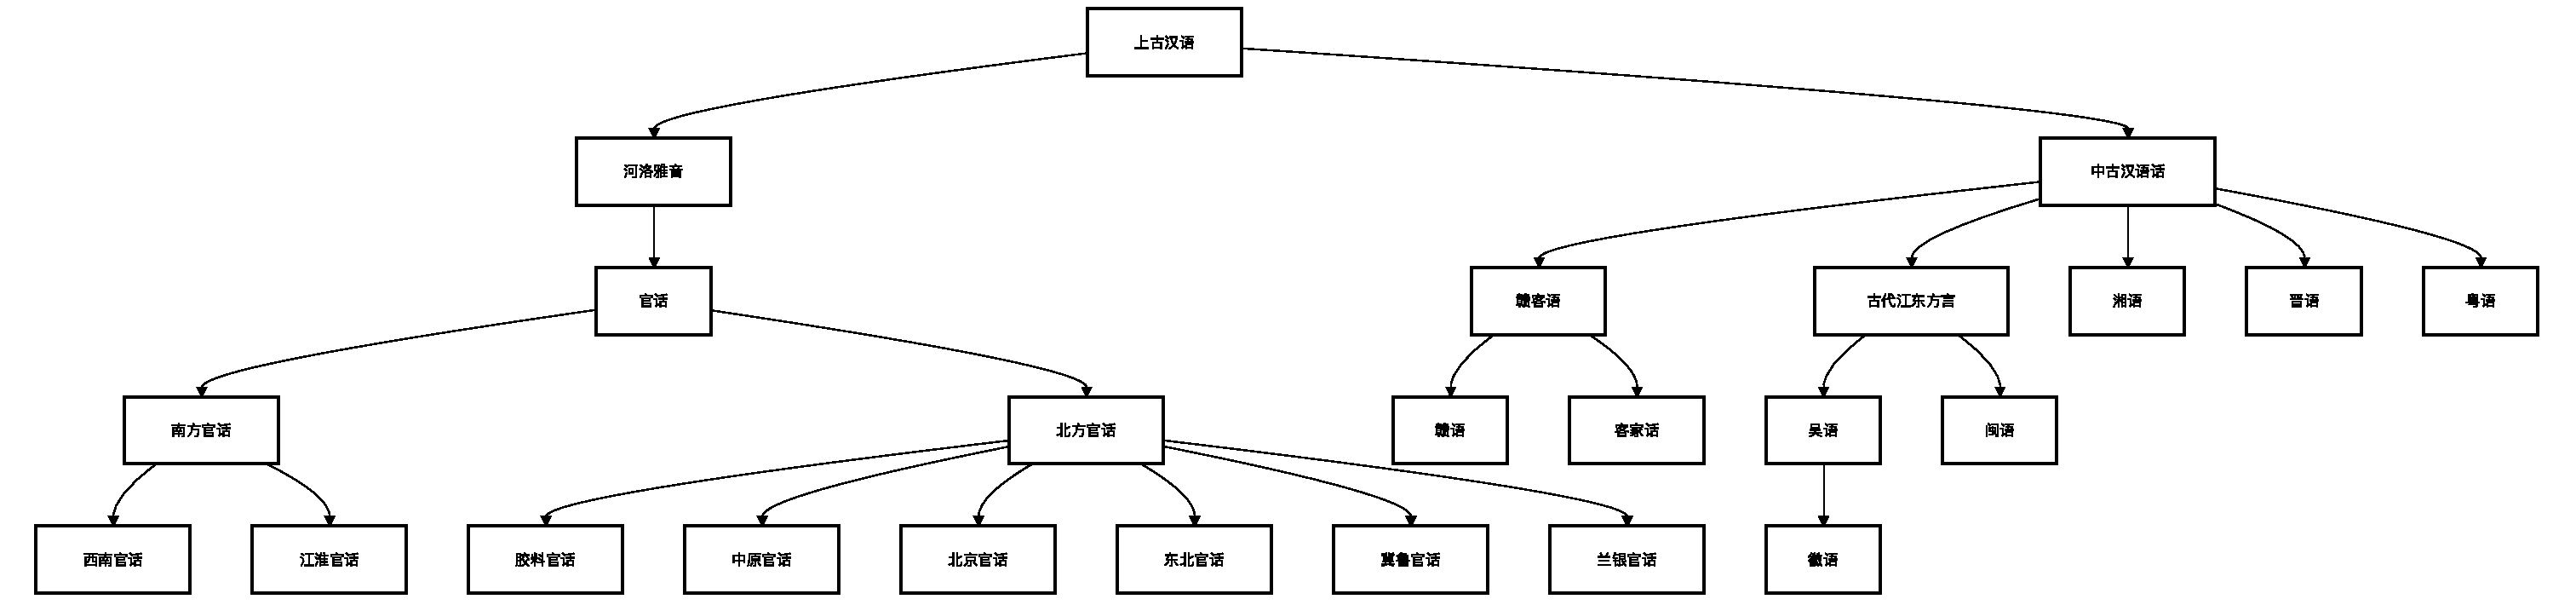
\includegraphics[width=\textwidth]{images/linguisitc_tree.drawio.pdf}
\end{figure}
由于各省之间存在大量的方言,并且现实中缺乏各方言在各省市中的人口分布数据,本文根据《中国语言地图集》选取各省的代表性语言作为其方言指标。值得注意的是部分省份由于内部存在大量完全分割的语言,例如江苏就包括吴语与江淮官话,本文选取流入人口较多的苏州、无锡一带的吴语作为其代表性语言;又例如山东省内部存在胶辽官话、冀鲁官话、中原官话,本文以济南市的冀鲁官话作为其代表性语言。本文的具体设置如表格\ref{tab:方言分布表}所示。
同时本文还将各省市的普通话普及率纳入模型,数据来源则参考了\cite{YuWeiQiGuoMinPuTongHuaNengLiDeJiBenZhuangKuangYuFaZhanTaiShi2018},从CGSS中获取。




\begin{table}[!ht]
\centering
\caption{方言分布表}
\begin{tabularx}{\textwidth}{@{}ccXccX@{}}
\toprule
\textbf{代表性方言} & \textbf{数量} & \multicolumn{1}{c}{\textbf{省份}} & \textbf{代表性方言} &\textbf{数量}  & \multicolumn{1}{c}{\textbf{省份}}\\
\midrule
西南官话 & 6 & 湖北省、广西壮族自治区、重庆市、四川省、贵州省、云南省 &晋语 & 2 &山西省、内蒙古自治区\\
东北官话 & 3 &辽宁省、吉林省、黑龙江省 & 北京官话  &1 &北京市\\
吴语 & 3 &浙江省、上海市、江苏省& 赣语  &1 &江西省\\
中原官话 & 3 &河南省、陕西省、青海省 &胶辽官话  &1& 山东省\\
冀鲁官话 & 2 &天津市、河北省、山东省 &湘语  &1 &湖南省\\
闽语 & 2 &福建省、海南省 &粤语  &1& 广东省\\
兰银官话 & 2 &甘肃省、宁夏回族自治区 &其他  &2& 西藏自治区、新疆维吾尔自治区\\
\bottomrule
\end{tabularx}
\label{tab:方言分布表}
\end{table}


本文对于复合指标的获取如表格所示

\section{方法上} % (fold)
\label{sub:方法上}

基于以上的推导,
在代码中需要先求出个体的似然,
而个体的总似然是迁移选择概率和工资观测概率的乘积,
那么集体的似然函数同时对未观测的随机效应(固定效应、地区匹配效应等)进行积分(离散求和):
\begin{equation}
  L_{i}=\sum\limits_{\text{所有随机效应组合}}[\prod_{t}\rho(x_{t},j_{t})\cdot P(w_{t}|\text{随机效应}) ]
\end{equation}

本文采用混合似然估计法(Mixed Likelihood Estimation)进行动态离散选择模型的参数求取。由于模型涉及高维状态空间与跨期动态关联性,计算过程具有三重复杂性:其一,个体选择行为需通过贝尔曼方程递归求解;其二,状态转移矩阵需处理多重内生性关联;其三,价值函数收敛需满足跨期一致性条件。

传统计量工具(如Stata)受限于矩阵运算效率与迭代算法架构,在应对此类包含200+状态变量、需进行10\^6量级矩阵运算的复杂场景时,存在计算耗时指数级增长与内存溢出的双重瓶颈。
为此,本文构建基于Python的数值计算框架,与传统的Stata相比,Python在实现复杂的动态离散选择模型方面具有显著优势:
首先,Python的开源生态系统提供了丰富的科学计算库,如\lstinline{NumPy}、\lstinline{Pandas}和\lstinline{PyTorch},这些库为处理大规模面板数据和实现复杂的优化算法提供了强大支持。特别是\lstinline{PyTorch}的自动微分功能,使得计算复杂模型的梯度变得简单高效,这在传统Stata环境中难以实现。
其次,Python的面向对象编程范式使得模型的各个组件可以被清晰地封装,提高了代码的可读性和可维护性。在本项目中,我们将模型的不同部分(如个体似然函数\lstinline{IndividualLikelihood}、参数估计器\lstinline{ModelEstimator}等)封装为独立的类,使得整体架构更加清晰。
此外,\lstinline{joblib}库提供的并行计算能力显著提高了计算效率,特别是在处理大量个体似然函数计算时;
本文设计逆向归纳算法(Backward Induction),通过倒序年龄迭代(从T期至$t_0$期)动态求解各状态节点的期望价值函数(EV矩阵),确保跨期决策路径的全局最优;
并运用SciPy优化器进行参数空间搜索,通过蒙特卡洛模拟生成选择概率曲面,最终实现模型参数在95\%置信区间内的有效估计。


对于求取参数的方法,传统上使用Newton线搜索方法上求解似然函数最大值,虽然收敛速度快,但计算海塞矩阵需要消耗大量资源。
虽然可以通过对似然函数进行LU分解,在计算海塞矩阵的逆时提供可靠帮助,降低数值不稳定性,
但计算海森矩阵的代价仍然较高,尤其是在参数较多时。
本文做出改进,
采取以自动微分(\lstinline{PyTorch})为核心,使用现代优化算法Quasi-Newton方法中的L-BFGS方法避免收敛困难和数值不稳定,并利用离散化与并行处理提升效率。
BFGS是一种拟牛顿法,通过迭代逼近目标函数的海塞矩阵的逆矩阵,从而避免直接计算二阶导数。它只需要利用梯度信息来更新海森矩阵的近似,使得每次迭代都能更准确地找到下降方向。在高维参数空间中,避免了直接计算海森矩阵的高计算成本。
在具体的梯度计算中,自动微分通过计算图追踪运算过程,利用链式法则自动计算导数,避免数值微分的截断误差。当模型复杂、参数众多,且需要频繁计算梯度时(如神经网络训练),自动微分显著优于手动编码梯度。对于需要高阶导数或大规模并行计算的情况尤为适合。
具体而言,
本文使用类方法分装待估参数
类继承
\lstinline{torch.nn.Module},所有参数为\lstinline{torch.nn.Parameter},支持自动梯度计算。

本文对于固定效应和地区匹配效应upsilon等支撑点离散化方法的处理与原作者的做法保持一致,
通过网格遍历求和。
对于已经用支撑点离散近似后的参数,在进行网格搜索时,
\lstinline{joblib.Parallel}支持将数据存储在磁盘上的内存映射文件中,这样多个进程可以共享同一份数据,
而无需每个进程都复制一份,从而显著降低内存消耗并提升 I/O 效率。

本文的优化方法基于深度学习,
模型估计结果对初始值存在一定敏感性,
初始值的选择可能会影响收敛速度和结果。例如,如果真实值接近-0.1,好的初始值能加快收敛。
虽然L-BFGS优化器在一定程度上缓解了这一问题,但仍需根据经济学理论进行初始值赋予能促进优化方法的应用,例如距离增加可能降低迁移概率,因此\lstinline{gamma_distance}的预期应该为负,将其初始值设为负符合理论预期,有助于引导优化方向。


本文中一些变量如表格\ref{tab:_实证与程序中的变量定义}所示。

\begin{table}
\centering
\caption{实证与程序中的变量定义}
\begin{tabularx}{\textwidth}{@{}ccXX@{}}
\toprule
变量符号 & 代码符号 & 含义 & 数据来源\\
\midrule
$\alpha_0$ & alpha0 & 经济性收入截距 &\\
$\alpha_1$ & alpha1 & 对于房价收入比作为宜居度的边际效用&\\
$\alpha_H$ & alphaH & 恋家溢价&\\
$\alpha_P$ & alphaP & 户籍制度惩罚&\\
$r_1$ & r1 & 年龄效应一次性系数& \\
$r_2$ & r2 & 年龄效应二次性系数& \\
 & houseprice & &\\
\bottomrule
\end{tabularx}
\label{tab:_实证与程序中的变量定义}
\end{table}

% ---------------------------------------- 估计结果 ----------------------------------------
\chapter{估计结果}

本文尝试回答一下几个问题:
\begin{itemize}
  \item 影响劳动力流动的因素是什么?到底哪些因素是负面因素(迁移摩擦)?
  \item 不同人群是否面对不同的劳动力迁移摩擦阻力?
  \item 本地的福利待遇对于迁移是否显著?这意味着是否可以通过政府补贴购买人才
  \item 
\end{itemize}


\cite{XiaYiRanChengShiJianDeMengMuSanQianGongGongFuWuYingXiangLaoDongLiLiuXiangDeJingYanYanJiu2015} 利用 2005 年 1\%人口抽样调查中劳动力流动的微观数据与 220 个地级市的城市特征 数据研究发现公共服务对劳动力流入产 生 吸 引 力,同 时 房 价 对 劳 动 力 流 入 也 有 正 向 作 用,他 们 认 为这是因为房价“资本化”了部分未观察到的公共服务或城市特征,此文关注点不在房价,而且使 用的普查 数 据 没 有 覆 盖 近 十 年 来 中 国 房 价 暴 涨 的 阶 段。

\section{基准回归与子样本分析} % (fold)


标准回归下得到的估计系数如下表格\ref{tab:基准回归系数}所示。
\begin{table}[!ht]
\centering
\caption{基准回归系数}
\begin{tabularx}{\textwidth}{@{}cXXX@{}}
\toprule
\midrule
\bottomrule
\end{tabularx}
\label{tab:基准回归系数}
\end{table}



McFadden’s Pseudo R²:用于快速评估模型解释力和向非技术受众展示结果。


农村劳动力回流存在吗?农村户口更容易回流吗?


\section{拟合优度} 

预测准确性 (Prediction Accuracy) 
要求模型能够准确地预测每个个体的选择行为或结果。
更关注局部性能(即单个样本的预测)。
可能对噪声敏感,尤其是在样本量较小或数据质量较差的情况下。

模拟校准 (Simulated Calibration) 
要求模型能够捕捉系统的整体动态特性,即使它无法完美预测单个样本的行为。
更关注全局性能(即整体数据的统计特性)。
对噪声相对不敏感,因为模拟校准关注的是长期趋势和分布特性。

\textbf{预测准确率(Prediction Accuracy)}

根据模型的预测结果与实际观测值进行比较,计算预测准确率或其他分类指标。

适用性:通过比较模型预测的选择概率与实际选择结果,计算正确预测的比例。直接评估模型的预测性能,尤其适用于分类问题。

常用指标:

- 准确率 (Accuracy): 预测正确的比例。

- 精确率 (Precision)、召回率 (Recall) 和 F1 分数。

- ROC 曲线下的面积 (AUC)。

优点:直观,特别适合评估模型在实际劳动力状态(如是否回流)预测中的表现。

缺点:可能过于简化,无法捕捉概率分布的细微差异,且对类别不平衡的数据敏感。

建议:在劳动力回流问题中,预测准确率可以作为辅助指标,特别是在政策分析中需要评估模型对回流决策的预测能力时。结合混淆矩阵(Confusion Matrix)可以进一步分析模型在不同状态(如回流 vs. 非回流)上的表现。


\textbf{模拟校准 (Simulated Calibration)}

定义 : 使用估计的模型参数生成模拟数据,并将模拟数据的统计特性(如均值、方差等)与实际数据进行比较。

用途 : 验证模型是否能够重现数据的关键特征。

局限性 : 需要额外的模拟步骤,计算成本较高。


\section{异质性人群的回归} 

其中关于经济性收入的参数,其估计结果如下表格\ref{tab:经济性参数的回归系数}所示。
\begin{table}[!ht]
\centering
\caption{经济性参数的回归系数}
\begin{tabularx}{\textwidth}{@{}cXXX@{}}
\toprule
\midrule
\bottomrule
\end{tabularx}
\label{tab:经济性参数的回归系数}
\end{table}


\section{从回归结果看待迁移摩擦}


\begin{table}[!ht]
\centering
\caption{迁移摩擦}
\begin{tabularx}{\textwidth}{@{}cXXX@{}}
\toprule
\midrule
\bottomrule
\end{tabularx}
\label{tab:迁移摩擦}
\end{table}



\section{迁移成本的具体构成}






% ---------------------------------------- 结论 ----------------------------------------
\chapter{结论与展望}

当然以城乡二元对立为代表的思想在我国依旧有非常重要的应用 因为我国依旧有大量依附于城乡关系的社会体系、福利体系等种种重要的制度
甚至在研究二元对立话题中依旧可以引入例如Rosen Roback这样的经典模型
例如 
\cite{GuoDongMeiChengXiangRongHeDeShouRuHeFuLiXiaoYingYanJiuJiYuYaoSuPeiZhiDeShiJiao2023}指出城乡融合的收入和福利效应研究——基于要素配置的视角
但对于在破除劳动力迁移摩擦、开放劳动力要素自由流动的当下
抛开这种二元对立的思想是越来越重要的
这也自然而然地引出了空间均衡与最有选址两种思路



由于普遍偏好事少离家近的特征,政策可以针对性地对周边省份进行补贴
相反 对于十分遥远地区的人力资源 即使补贴了显性的迁移成本 也存在较长的文化、心里距离 所以在边际上可能并不值得投入



本文可以改进的地方:

添加约束

添加宏观变量

使模型作为微观基础从而宏观化
\textit{近年来,一些研究将上述两种基础模型结合起来,在空间均衡模型中加入了微观层面的动态迁移决策特征。这些动态一般均衡迁移模型明确考虑了空间工资差异的来源及其对净迁移和总迁移的影响,并允许存在不同类型的空间障碍,如劳动力重新配置摩擦和信息摩擦。这类模型特别关注迁移如何作为调节各地劳动力市场长期均衡的机制。例如,Coen-Pirani(2010)开发了一个动态一般均衡模型,强调了个体迁移决策中的不可观测异质性。该模型刻画了总迁移流动和净迁移流动的共同模式,其中前者由个体匹配的偶然冲击驱动,后者由持续的生产率冲击驱动。工人会迁移到正受到生产率冲击的地区,并在迁移后发现其偶然匹配的质量。新迁移的工人比长期居住者更可能继续迁移,因为后者选择留在某地是由于他们已经获得了相对较好的匹配。该校准模型可以解释为何人口流入较多的地区往往也伴随着较多的流出,这一现象在仅研究净流入的模型中无法得到解释。结合偶然匹配效应的空间均衡模型还能够解释新迁入工人与迁出工人在年龄、教育和行业等方面的相似性,这些特征无法仅通过个体位置选择模型或仅基于可观测工人异质性或地点特定冲击的模型来解释。}

从而引入其他变量

以家庭为基本单位


% ---------------------------------------- 附录 ----------------------------------------
\newpage
\appendix

\chapter{McFadden条件概率}

个体选择选项j的条件是其总效用最大,即
$u_j + \zeta_j > u_k + \zeta_k, \forall k \neq j$。
这可以转化为
$\zeta_j - \zeta_k > u_k - u_j, \forall k \neq j$。
假设误差项$\zeta_j$独立且服从相同的极值分布,则对于每个$k \neq j$,有
$\Pr(\zeta_j > \zeta_k + (u_k - u_j)) = \frac{1}{1 + \exp(u_k - u_j)}$。
在RUM模型中,当误差项独立时,选择j的概率为所有选项k的独立事件同时发生的概率,即
$P_j = \prod\limits_{k \neq j} \Pr(\zeta_j > \zeta_k + (u_k - u_j))$。
代入单个事件的概率表达式,选择j的概率是所有$k \neq j$的条件概率的乘积
$P_j = \prod\limits_{k \neq j} \frac{1}{1 + \exp(u_k - u_j)}$。
对$P_j$取对数
$\ln P_j = - \sum_{k \neq j} \ln(1 + \exp(u_k - u_j))$。
通过指数函数的性质,将上述表达式转换为
$P_j = \frac{\exp(u_j)}{\sum\limits_{k \in C} \exp(u_k)}$。

\chapter{效用等价于收入的特殊情况}
假设效用函数的线性形式为$U(x)=a X$,其中a为边际效用参数。居民可在固定利率$r$下无限制借贷,预算约束满足消费现值等于收入现值。
居民可以留在原地(永久收入为$Y_h$)或迁移(永久收入为$Y_p$,后者需支付一次性迁移成本 $M$。
假设迁移成本 
$M$
为即期支出,且永久收入为永续年金。

若居民留在原地,其永久收入的现值为
$W_h = \sum\limits_{t=0}^\infty \frac{Y_h}{(1+r)^t}=\frac{Y_h}{r}$,
总效用为$U_h=a W_h = \frac{a Y_h}{r}$。
若居民选择迁移,需支付即期成本 
$M$
,迁移后的永久收入现值为
$W_h = \sum\limits_{t=0}^\infty \frac{Y_p}{(1+r)^t}=\frac{Y_p}{r}$,
由于迁移成本 
$M$
为即期支出,净现值为
$\mathcal{W}=W_p-M=\frac{Y_p}{r}-M$,
总效用为
$U_p=a(\frac{Y_p}{r}-M)$
迁移的条件为$U_p>U_h \Rightarrow a(\frac{Y_p}{r}-M) > a \frac{ Y_h}{r} \Rightarrow Y_p-Y_h > rM$。
期望效用最大化等价于选择净现值更高的选项,即$\max{a(\frac{Y_p}{r}-M), a \frac{ Y_h}{r}}$。

\chapter{Rust极值分布}
公式中的随机效用项假设服从于一类极值分布
We assume that $\zeta_j$ is drawn from the Type I extreme value distribution. In this case, using arguments due to McFadden (1973) and Rust (1987), we have
$$\exp\left(\bar{v}(x)\right) = \sum_{k=1}^J \exp\left(v(x, k)\right)$$

这表示如果变量服从一类极值分布,那么$\exp\left(\bar{v}(x)\right)$可以表示为所有$v(x, k)$的指数和
它意味着,在状态x 下,选择某一选项j的概率与效用的指数值成比例。
这个性质广泛用于预测个体选择的分布。

\chapter{地点选择概率}
$\rho(x,j)=\frac{\exp(v(x,j))}{\sum\limits_{k=1}^{J} exp(x,k)}$

Probability that a person in state $x$ will choose location $j$ can then be written as
$$\rho(x,j)=\exp[v(x,j)-\bar v(x)]$$
% section 附录_证明 (end)证明

\chapter{log} % (fold)

令$\mathcal{K}_{it}=(\mathcal{K}_{it}^{0},\mathcal{K}_{it}^{1})$表示当前位置和上一个位置

已知\ref{eq:地点选择概率},
个体i在t时期选择目的地的似然概率是$\lambda_{it}(\omega^{i},\theta_{\tau})$
同时在
\begin{equation}
  \lambda_{it}(\omega^{i},\theta_{\tau})=\rho(x,j)=\rho_{h(i)}(\ell(i,t),\omega_{\nu}^{i}(\mathcal{K}_{it}^{0}),\omega_{\nu}^{i}(\mathcal{K}_{it}^{1}),\omega_{\xi}^{i}(\mathcal{K}_{it}^{0}),\omega_{\xi}^{i}(\mathcal{K}_{it}^{0}),a_{it},\ell^{0}(i,t+1),\theta_{\tau})
\end{equation}
公式表明个体的选择不仅受到过去历史(如上一个地点和上一个选择)和随机效应(如匹配效应和暂态效应)的影响,还考虑了个体的长期偏好和未来选择的影响。
通过对这个似然函数进行建模,我们可以估计个体在特定情况下做出选择的概率,从而理解个体在复杂环境下如何做出决策。


由于暂态效应服从期望为$0$的正态分布,并且已知经济收益函数设定为公式\ref{eq:经济收益函数},
令$\Psi$表示标准正态分布的概率累积函数,$\phi$表示标准正态分布的概率密度函数,可知经济收益函数的密度函数为
\begin{equation}
  \Psi_{it}(\omega^{i},\theta)=\phi(\frac{w_{it} - \mu_{\ell^{0}(i,t)}-G(X_{i},a_{it},\theta)-\nu(\omega_{nu}^{i}(\mathcal{K}_{it}^{0}))-\eta(\omega_{\eta}^{i})  }{\sigma_{\epsilon}(\omega_{\epsilon}^{i})})
\end{equation}
其中$\mu_{\ell^{0}(i,t)}$:是个体i在位置$\ell$基础工资水平;$G(X_i, a_{it}, \theta)$:代表个体$i$在时间$t$受到的外部影响(如经济环境、工作特征等);$\nu(\omega_{\nu}^i(\mathcal{K}_{it}^0))$、$\eta(\omega_{\eta}^i)$:分别是地区匹配效应和固定效应,它们是收入的随机组成部分,影响个体的收入;$\sigma_{\epsilon}(\omega_{\epsilon}^i)$:表示暂态效应的标准差,它反映了短期收入波动的程度。

这是在时期$t$给定个体$i$的选择和随机效应(如匹配效应、固定效应等),观察到收入$w_{it}$的概率概率,即被观测收入的似然概率。


\chapter{a}


To specification, factors including but not limited to as follow:

- income improvement. Higher income by comparison induces migration. 

- house price. Most researches agree the effect coulde be U-shaped.

- public service is a very large genre, we try to avoid such big word. It is a combination of all kinds of government-provided goods and natural resources. And the richer diveristy and better quality local government can provide, more migration is induced.

- weather

- hazzards

- cultural barrier is another big word genre, including but not limited to language barrier, habits, identity recognition and 

- direct migration cost, a total amount of present money paid for the transfer from one place to another. 迁移成本模型: 迁移成本模型考虑了个体在选择居住地时需要支付的成本(如搬家费用、适应新环境的成本等)。在考虑这些成本的情况下,个体可能会选择效用次优的居住地以避免高迁移成本。


\newpage
\bibliography{Papers}
\bibliographystyle{gbt7714-plain}
% \bibliographystyle{gbt7714-author-year}
\end{document}
